\renewcommand{\appendixname}{Anexo}
\renewcommand{\thechapter}{\Alph{chapter}}

% Comando para iniciar la sección de anexos en el índice
\newcommand{\initappendix}{%
  \addcontentsline{toc}{chapter}{Anexo}%
}

% Comando para cada anexo individual
\newcommand{\anexo}[1]{%
  \refstepcounter{chapter}%
  \chapter*{Anexo \thechapter: #1}%
  \addcontentsline{toc}{section}{Anexo \thechapter: #1}%
  \markboth{Anexo \thechapter: #1}{}%
}

\initappendix

% Anexos. En la entrega final el cronograma no va: se quita su \input y los
% demás anexos se renumeran solos (todas las menciones usan \ref).
% \anexo{Cronograma}\label{annex:diagramas}

El cronograma complementa la tabla de sprints de la Subsubsección~\ref{subsec:sprints}. La Figura~\ref{fig:gantt} reúne las etapas, sus duraciones y los hitos de control de la cátedra; las barras representan planificación, no evidencia de ejecución.
% Diagrama de Gantt del Proyecto Final de Ingeniería.
% Cronograma de marzo a diciembre de 2026 con desglose semanal: cada mes se
% divide en 4 columnas (40 slots en total), de modo que las barras pueden
% comenzar y terminar en semanas concretas y no en meses enteros.
% Alineado con el cronograma oficial de la cátedra de PFI:
%   - 25/04: entrega de la propuesta de tema        -> semana 8.
%   - 13/06: entrega del avance del 25 %            -> semana 14.
%   - 22/08: exposición del avance del 50 %         -> semana 24.
%   - 24/10: entrega del informe escrito (75 %)     -> semana 32.
%   - 09-14/12: defensa del PFI (llamado regular)   -> semana 38.
% Los grupos (\ganttgroup) reúnen los ítems a evaluar en cada una de las
% entregas restantes (50 %, 75 % y final), según la devolución del avance
% del 25 %. Ajustar barras e hitos a medida que avance el proyecto.
\begin{figure}[ht]
	\centering
	\resizebox{\textwidth}{!}{%
		\begin{ganttchart}[
			x unit=0.45cm,
			hgrid,
			vgrid={*3{draw=none}, dotted},
			bar/.append style={fill=NavyBlue!60},
			bar height=0.6,
			bar label font=\small,
			group label font=\small\bfseries,
			title label font=\small,
			milestone/.append style={fill=BrickRed},
			milestone label font=\footnotesize\itshape,
			milestone left shift=-0.5,
			milestone right shift=-0.5,
			y unit title=0.55cm,
			y unit chart=0.6cm
			]{1}{40}
			\gantttitle{2026}{40} \\
			\gantttitle{Mar}{4}\gantttitle{Abr}{4}\gantttitle{May}{4}\gantttitle{Jun}{4}\gantttitle{Jul}{4}\gantttitle{Ago}{4}\gantttitle{Sep}{4}\gantttitle{Oct}{4}\gantttitle{Nov}{4}\gantttitle{Dic}{4} \\

			% Etapas generales (semanas 1-40)
			\ganttbar{Propuesta de tema}{1}{8} \\
			\ganttbar{Marco teórico y Estado del Arte}{5}{18} \\
			\ganttbar{User Research (encuesta y entrevistas)}{9}{22} \\
			\ganttbar{Redacción del documento}{5}{34} \\
			\ganttmilestone{Propuesta de tema (25/4)}{8} \\
			\ganttmilestone{Avance 25\% (13/6)}{14} \\

			% Ítems a evaluar en el avance del 50 % (22/8)
			\ganttgroup{Ítems del avance 50\%}{13}{24} \\
			\ganttbar{Diseño y arquitectura del sistema}{13}{20} \\
			\ganttbar{Metodología de desarrollo (Sec. 4)}{15}{22} \\
			\ganttbar{Cierre del User Research (Sec. 3.1)}{17}{23} \\
			\ganttmilestone{Avance 50\% (22/8)}{24} \\

			% Ítems a evaluar en el avance del 75 % (24/10)
			\ganttgroup{Ítems del avance 75\%}{21}{32} \\
			\ganttbar{Desarrollo del prototipo (MVP)}{21}{30} \\
			\ganttbar{Integración de fuentes de datos}{25}{31} \\
			\ganttbar{Pruebas y validación (Sec. 5)}{27}{32} \\
			\ganttmilestone{Avance 75\% (24/10)}{32} \\

			% Ítems de la entrega final y defensa
			\ganttgroup{Ítems de la entrega final}{33}{39} \\
			\ganttbar{Discusión y conclusiones (Secs. 6 y 7)}{33}{35} \\
			\ganttbar{Resumen, abstract y correcciones finales}{34}{37} \\
			\ganttbar{Preparación de la defensa}{36}{39} \\
			\ganttmilestone{Defensa (9--14/12)}{38}
		\end{ganttchart}%
	}
	\caption{Diagrama de Gantt con el cronograma del proyecto. Fuente: elaboración propia.}
	\label{fig:gantt}
\end{figure}

            % Cronograma (solo entregas parciales)
\anexo{Pantallas y wireframes de Allocia}\label{annex:wireframes}

Este anexo completa la Subsección~\ref{sec:pantallas} con las pantallas del cliente web que no aparecen en el cuerpo del Proyecto y con los wireframes de alta fidelidad del diseño original, en formato móvil, elaborados con Stitch (Google). Las capturas provienen de una cuenta de prueba con ocho posiciones, con el correo difuminado donde aparece: acceso y registro (Figura~\ref{fig:anx-acceso}), el cliente web en el navegador de un teléfono (Figura~\ref{fig:anx-web-movil}), política de privacidad y cuenta con exportación y baja (Figura~\ref{fig:anx-privacidad}), desglose y detalle por activo (Figura~\ref{fig:anx-desglose}), alertas e informe (Figura~\ref{fig:anx-alertas}) y ajustes (Figura~\ref{fig:anx-ajustes}). En la Figura~\ref{fig:anx-acceso}, las tarjetas de la ilustración lateral son de demostración.

\section*{Pantallas del cliente web}
\begin{figure}[ht]
	\centering
	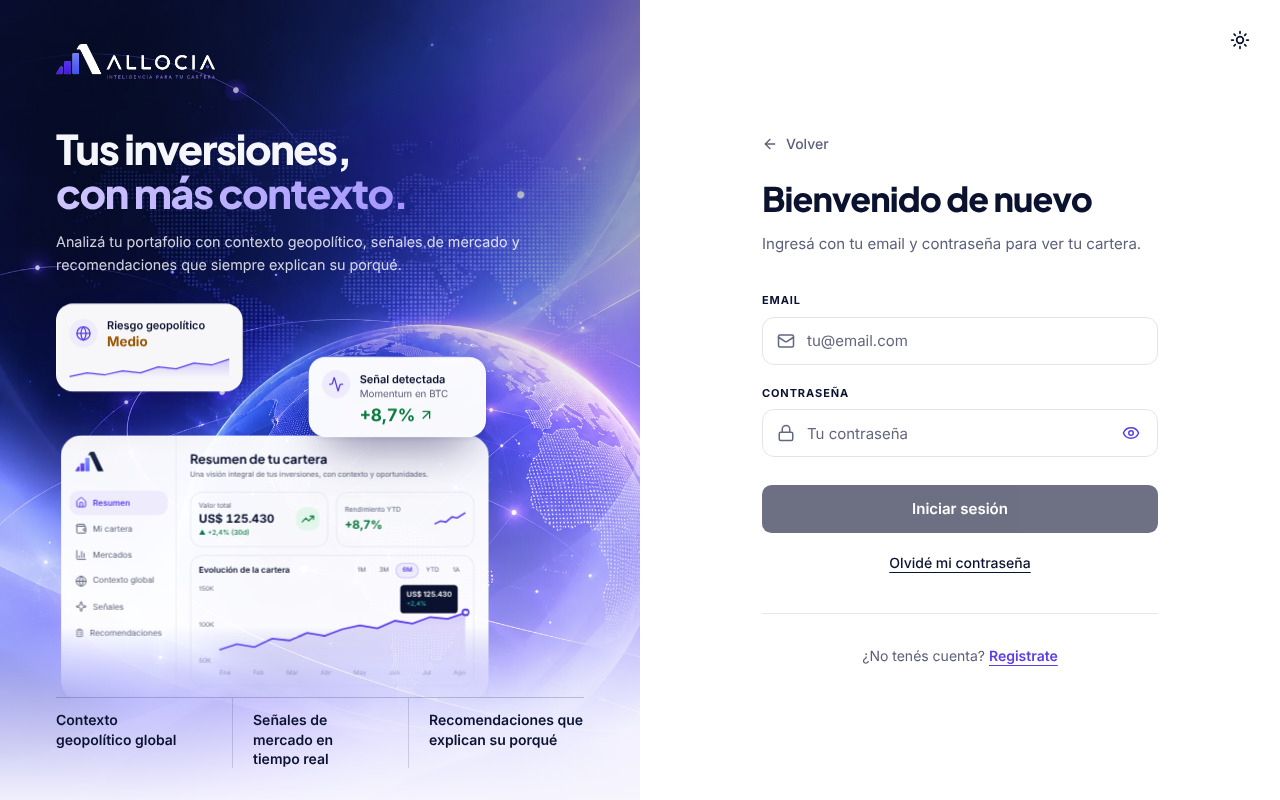
\includegraphics[width=0.485\textwidth]{figures/pantallas/web/a-02-login.png}\hfill
	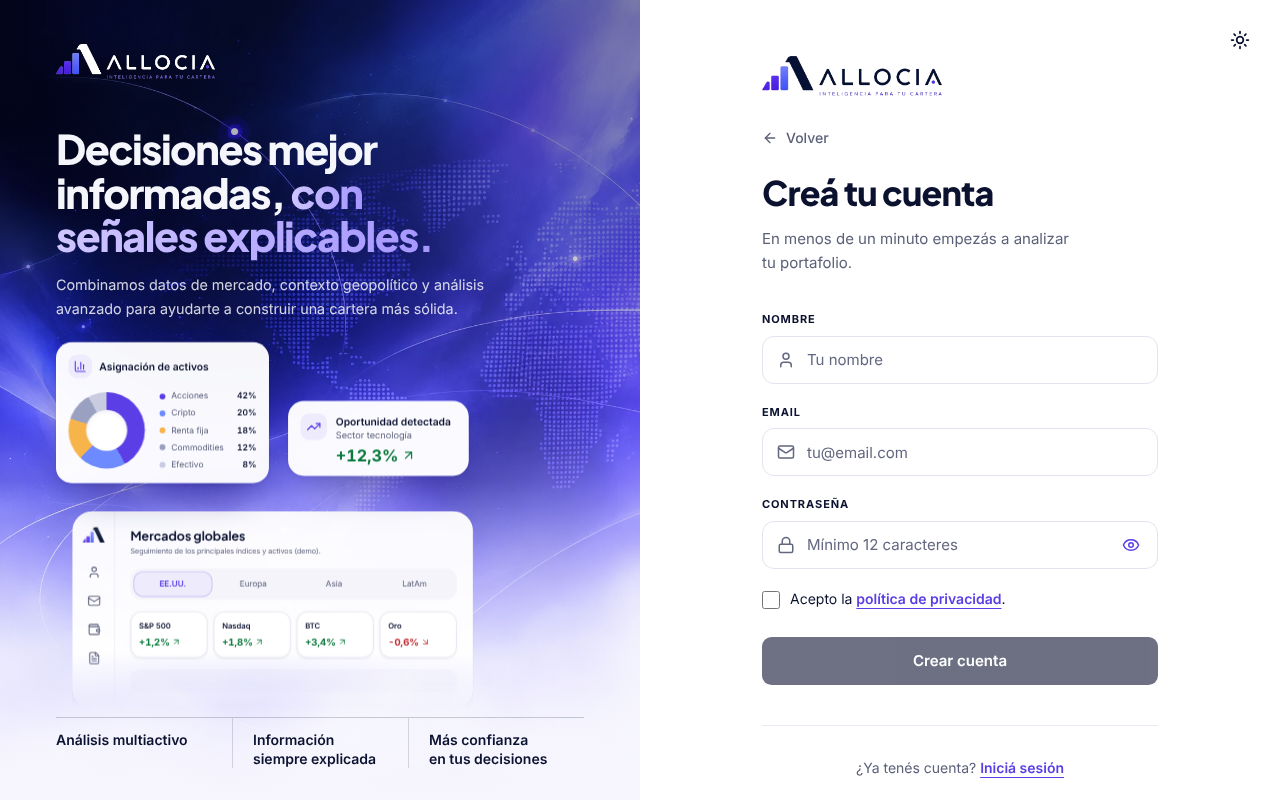
\includegraphics[width=0.485\textwidth]{figures/pantallas/web/a-03-registro.png}
	\caption{Capturas del inicio de sesión y del registro. Fuente: elaboración propia.}\label{fig:anx-acceso}
\end{figure}

\section*{Cliente web en el teléfono}
El cliente web adapta su diseño a la pantalla de un teléfono: el menú lateral se reemplaza por una barra de pestañas inferior y las tarjetas se apilan en una sola columna. La Figura~\ref{fig:anx-web-movil} muestra Resumen, Riesgo y Señales en el navegador de un teléfono, sin la aplicación instalada.
\begin{figure}[ht]
	\centering
	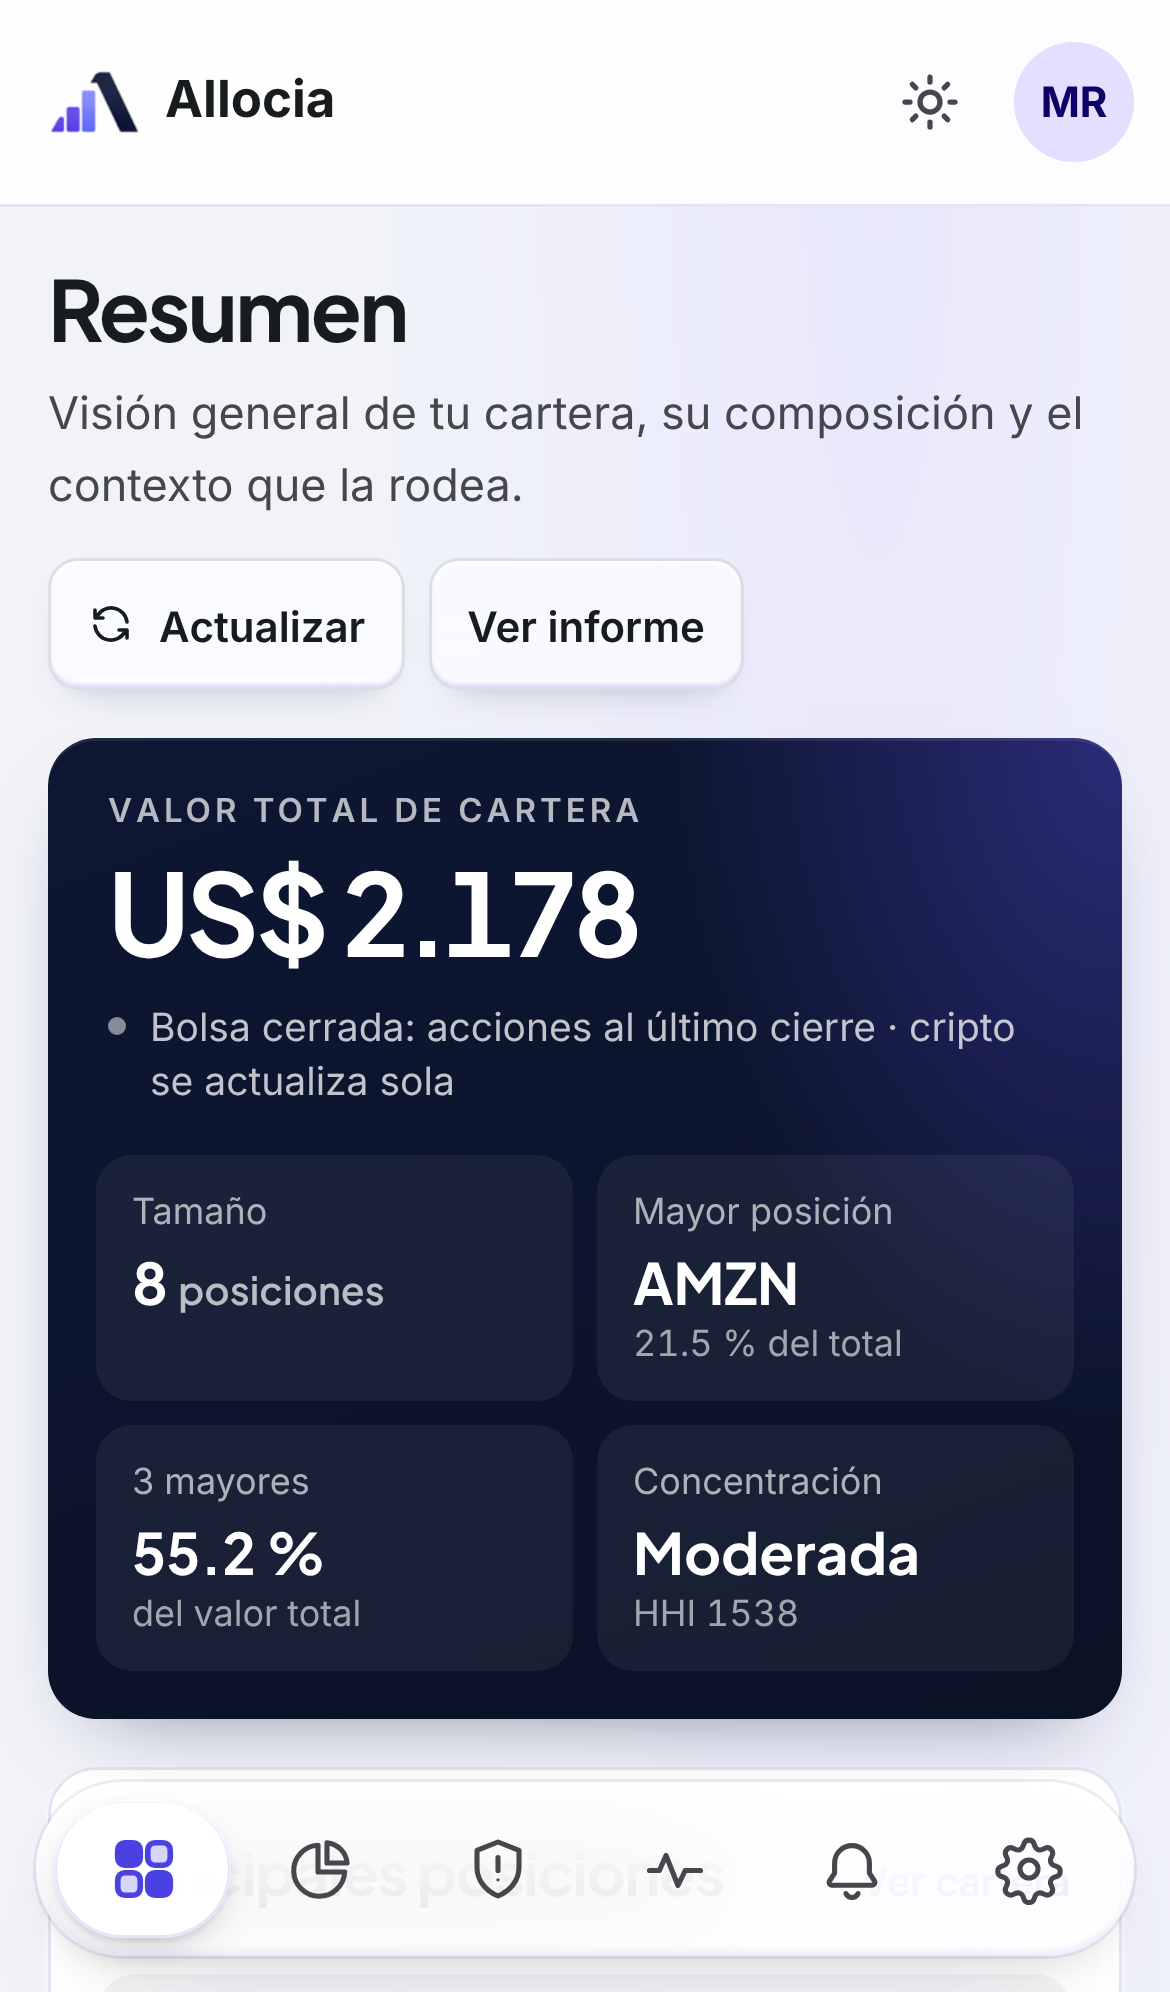
\includegraphics[height=7.4cm]{figures/pantallas/web/m-01-resumen.png}\hspace{4pt}
	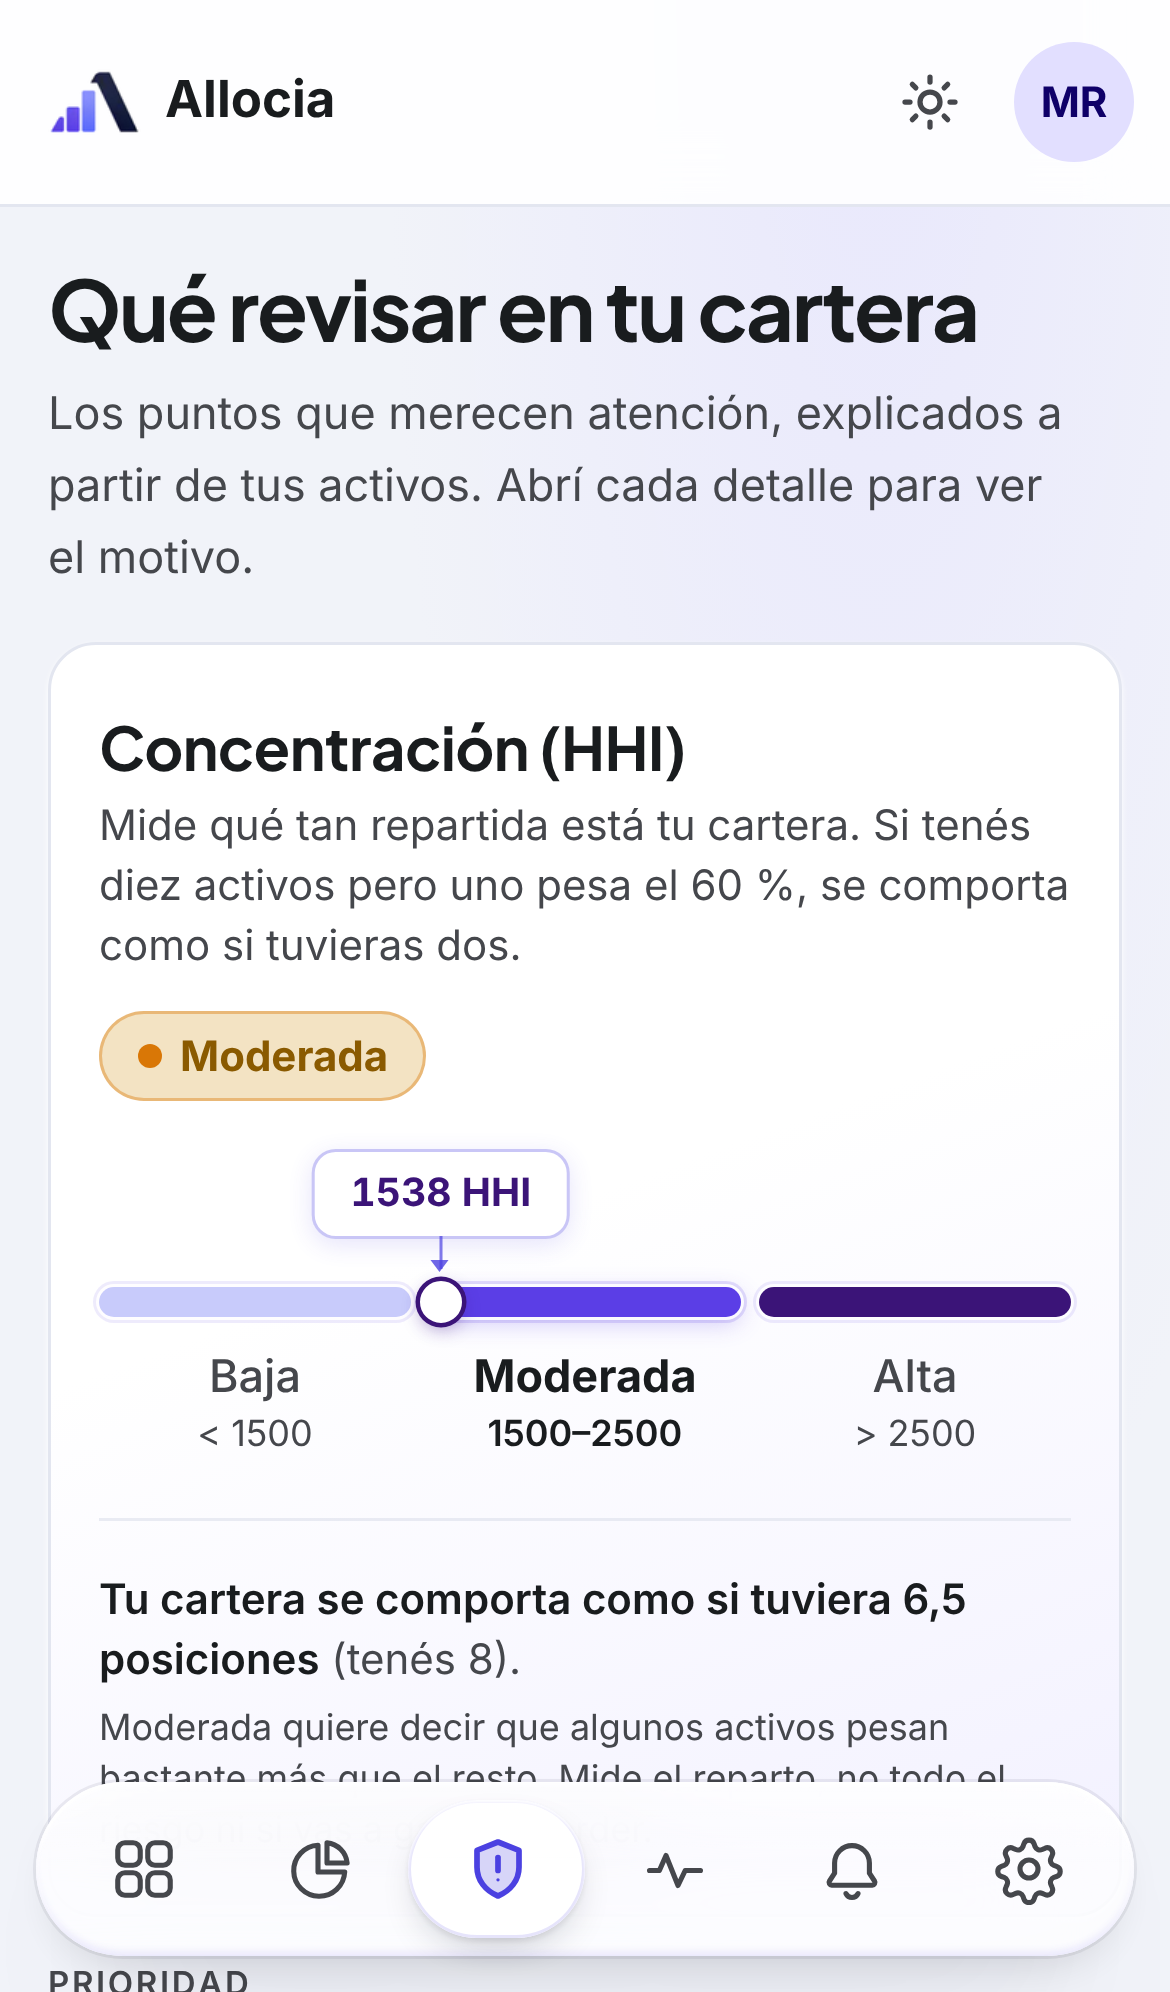
\includegraphics[height=7.4cm]{figures/pantallas/web/m-02-riesgo.png}\hspace{4pt}
	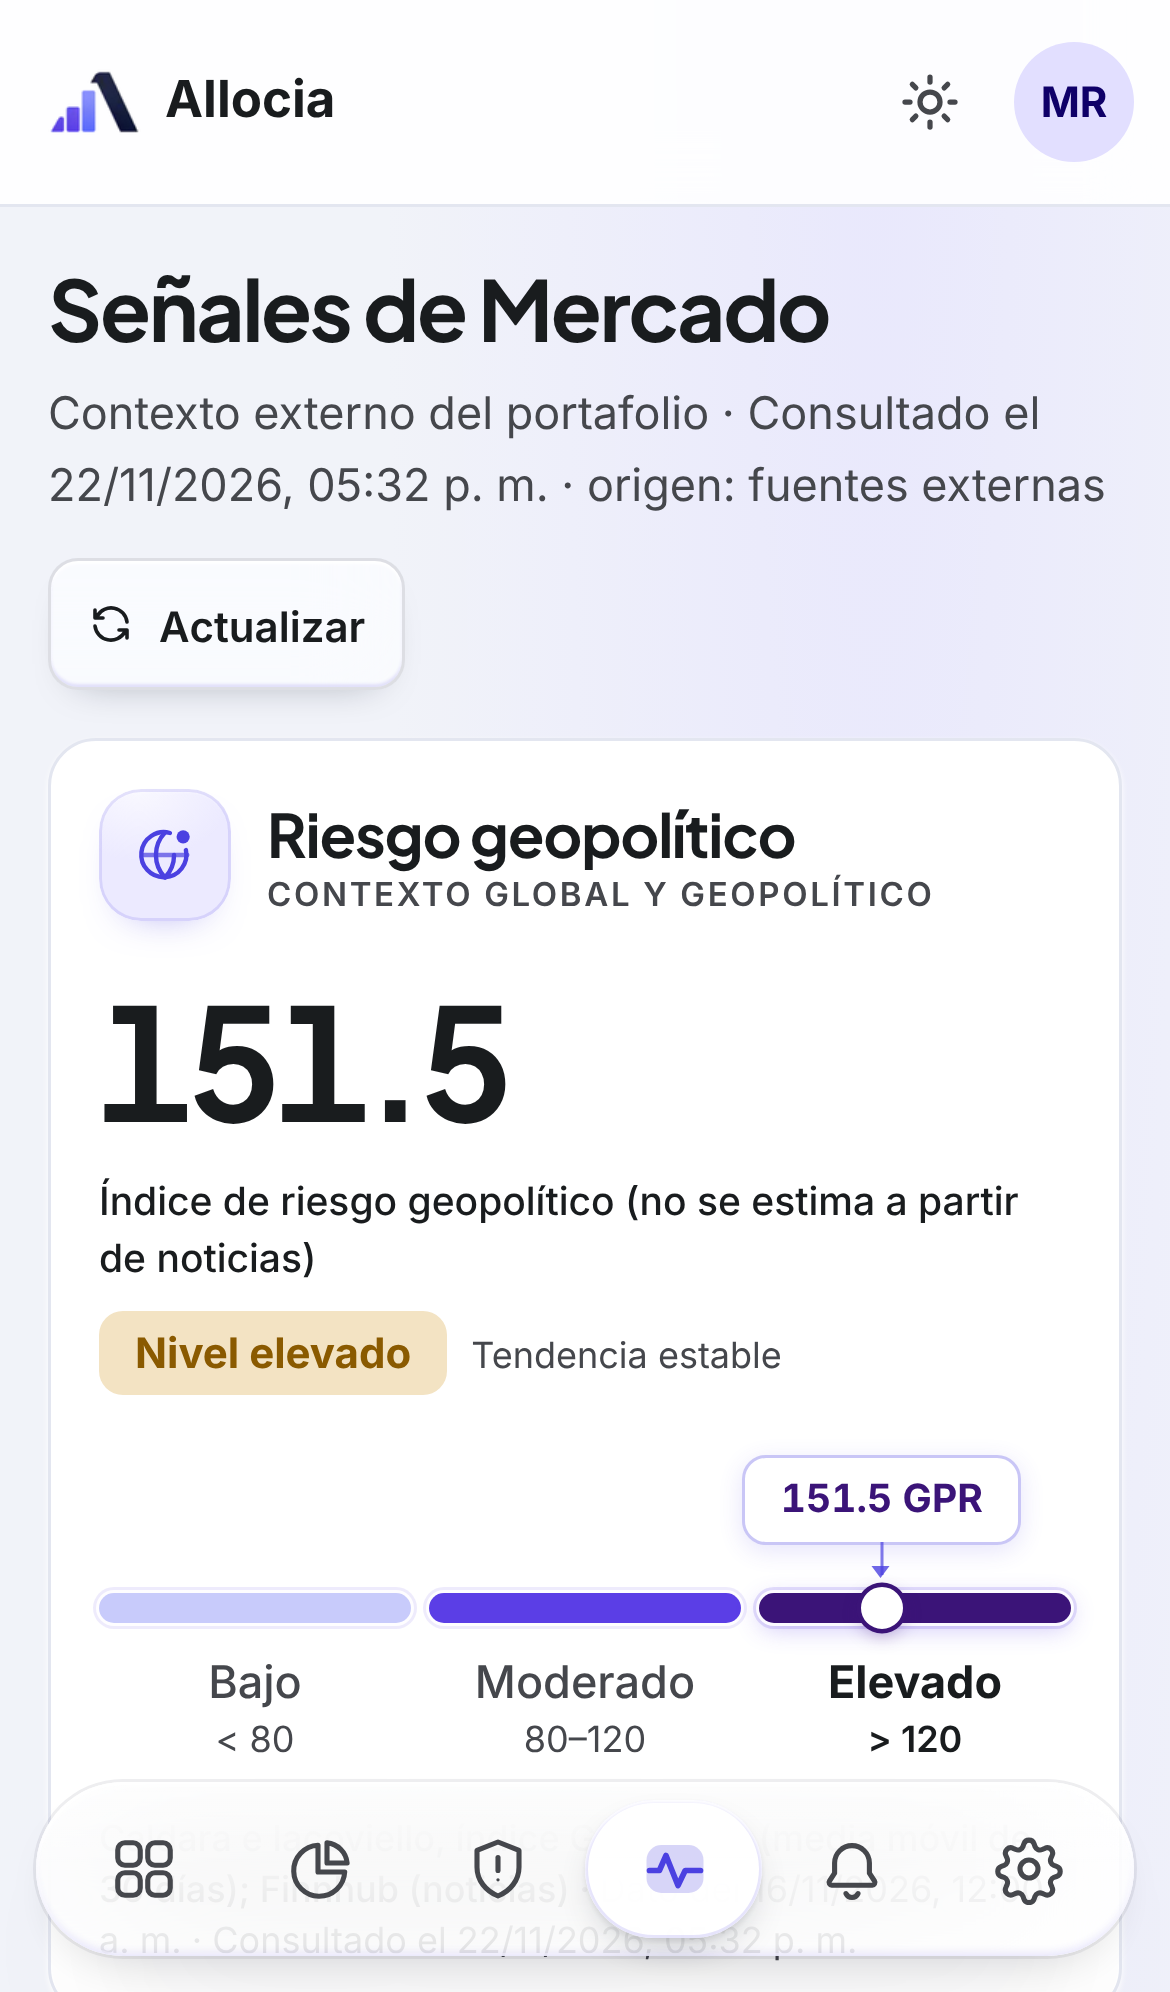
\includegraphics[height=7.4cm]{figures/pantallas/web/m-03-senales.png}
	\caption{Capturas del cliente web en el navegador de un teléfono: Resumen, Riesgo y Señales. Fuente: elaboración propia.}\label{fig:anx-web-movil}
\end{figure}

\section*{Privacidad y baja de cuenta}
La política de privacidad indica quiénes son los responsables, con qué finalidad se tratan los datos, cuáles se tratan, cuánto tiempo se guardan y qué derechos tiene la persona. La pantalla de cuenta permite exportar los datos y pedir la baja confirmando la contraseña (RF9 y RF10). La propia política aclara que un responsable legal debe revisarla antes de publicar el servicio.
\begin{figure}[ht]
	\centering
	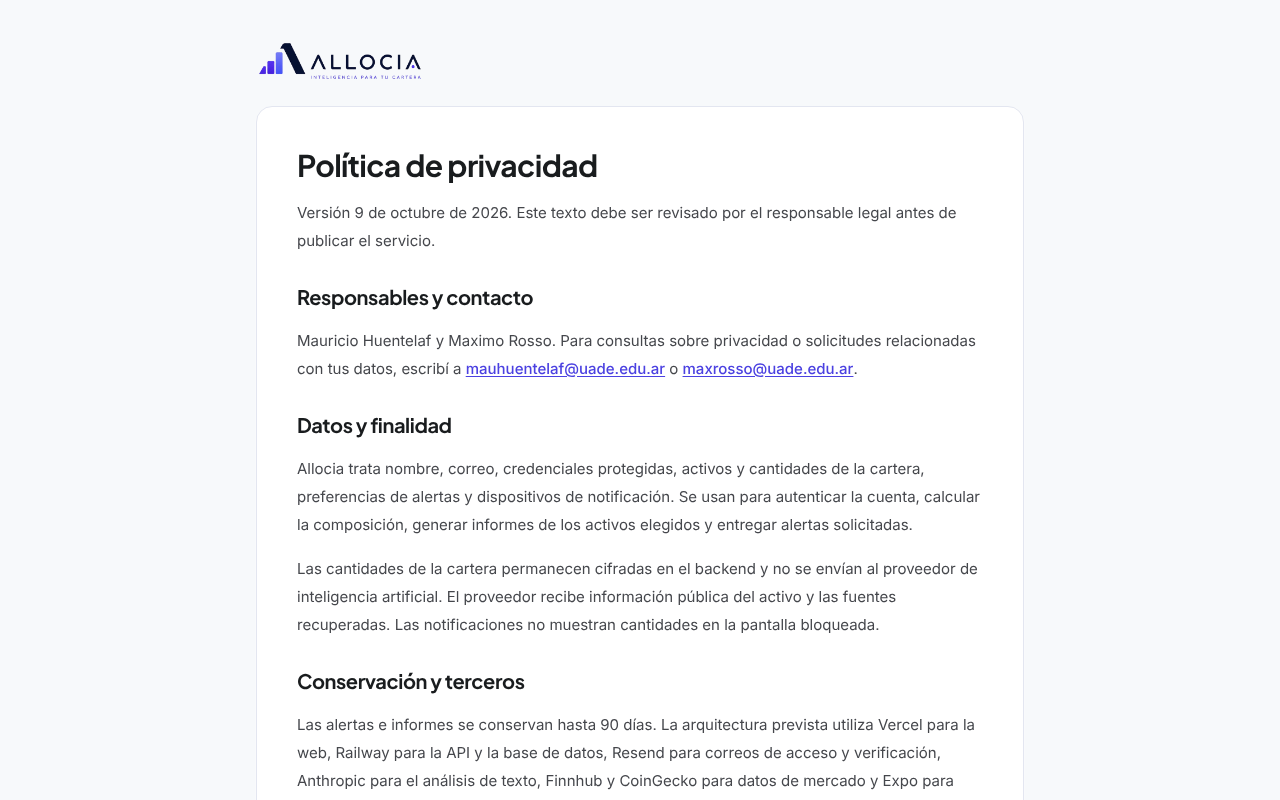
\includegraphics[width=0.82\textwidth]{figures/pantallas/web/a-04-privacidad.png}\\[6pt]
	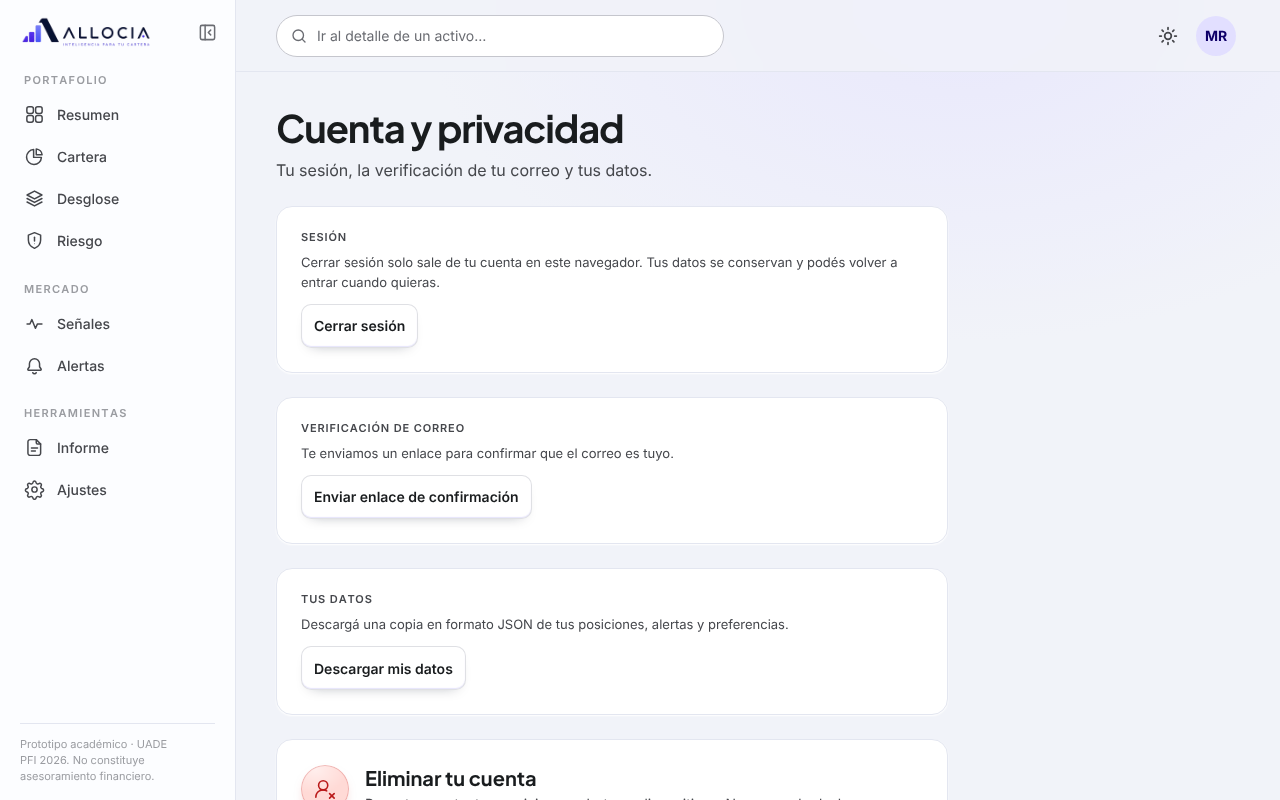
\includegraphics[width=0.82\textwidth]{figures/pantallas/web/a-10-cuenta.png}
	\caption{Capturas de la política de privacidad y de la pantalla de cuenta, con exportación y baja. Fuente: elaboración propia.}\label{fig:anx-privacidad}
\end{figure}

\begin{figure}[ht]
	\centering
	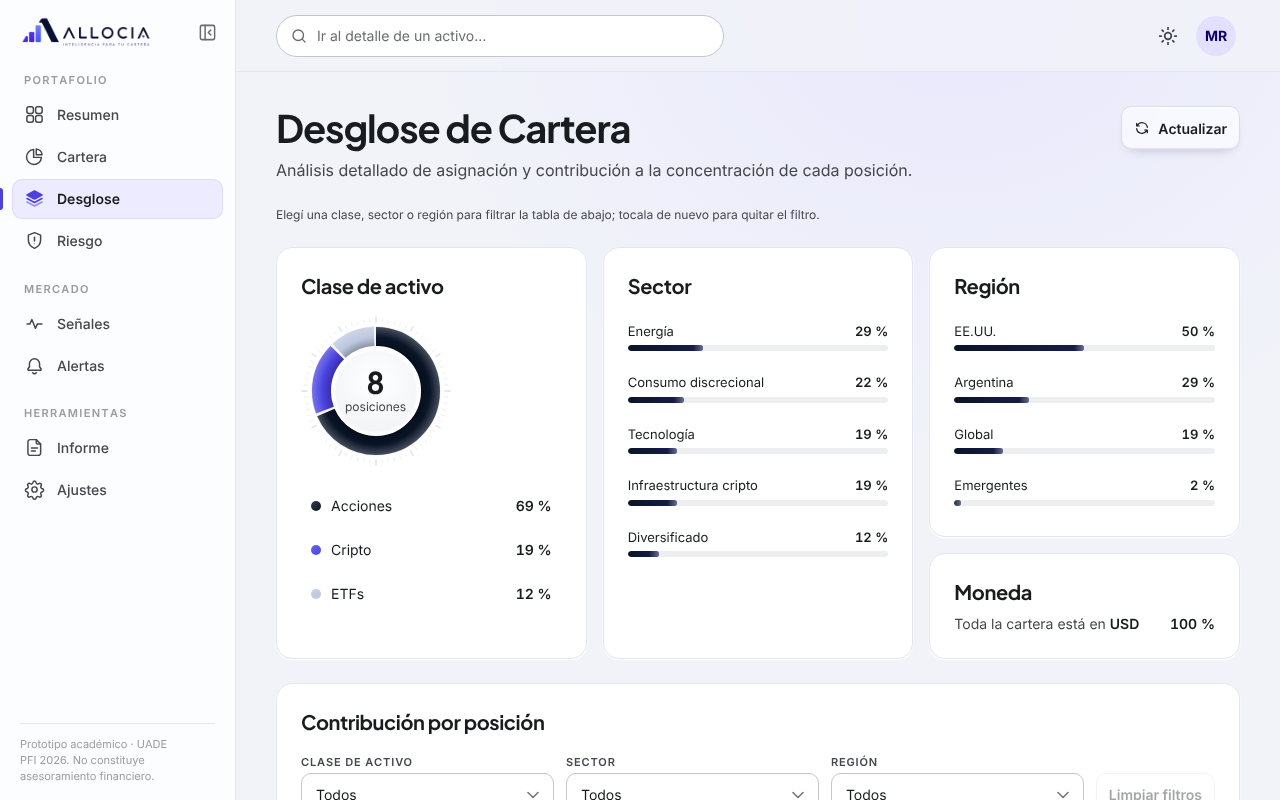
\includegraphics[width=0.82\textwidth]{figures/pantallas/web/a-05-desglose.png}\\[6pt]
	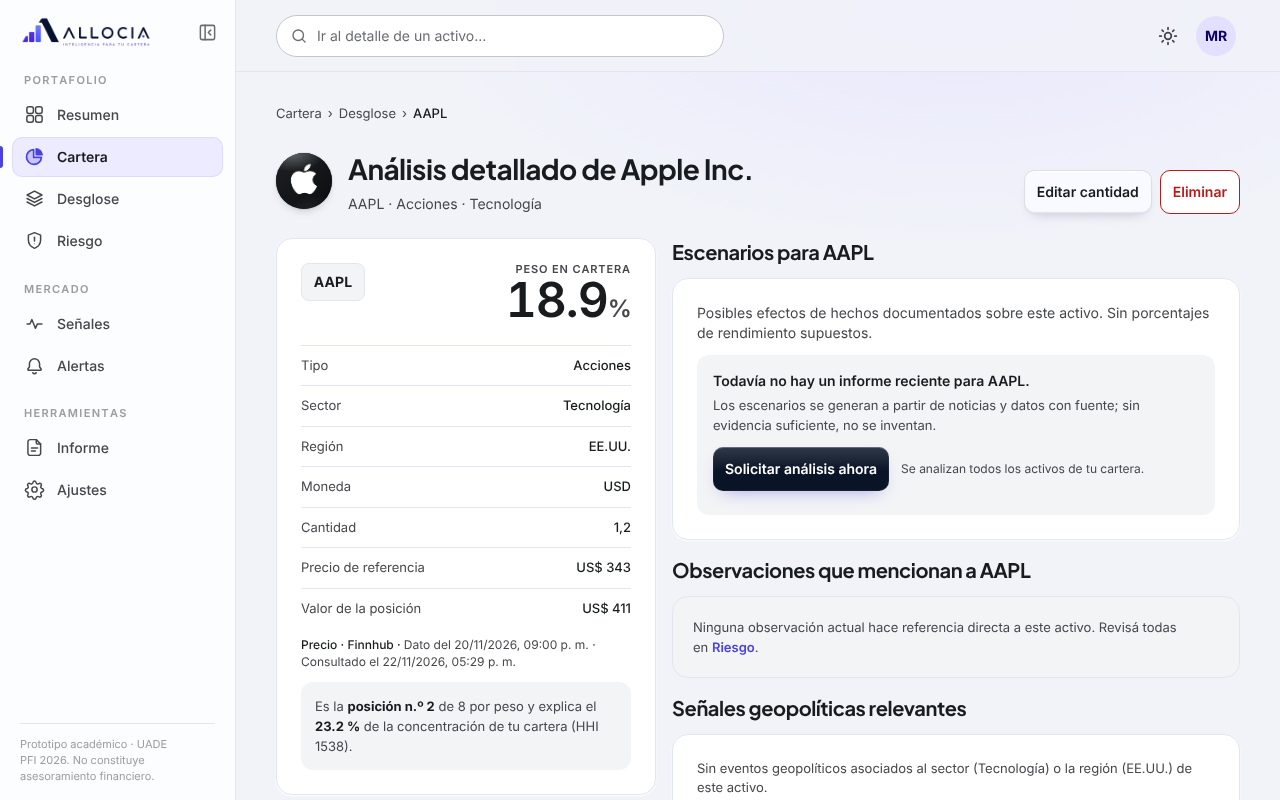
\includegraphics[width=0.82\textwidth]{figures/pantallas/web/a-06-detalle.png}
	\caption{Capturas del desglose de la cartera y del detalle de un activo. Fuente: elaboración propia.}\label{fig:anx-desglose}
\end{figure}

\begin{figure}[ht]
	\centering
	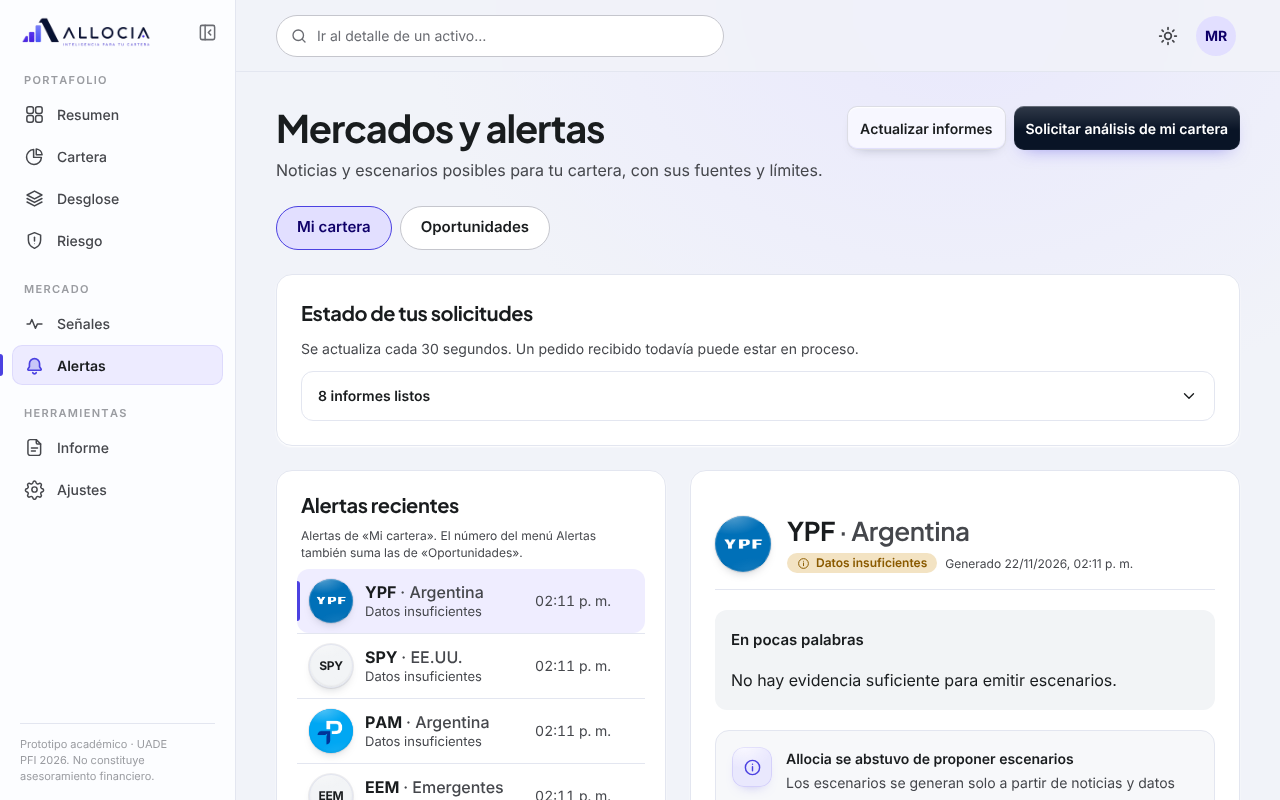
\includegraphics[width=0.82\textwidth]{figures/pantallas/web/a-07-alertas.png}\\[6pt]
	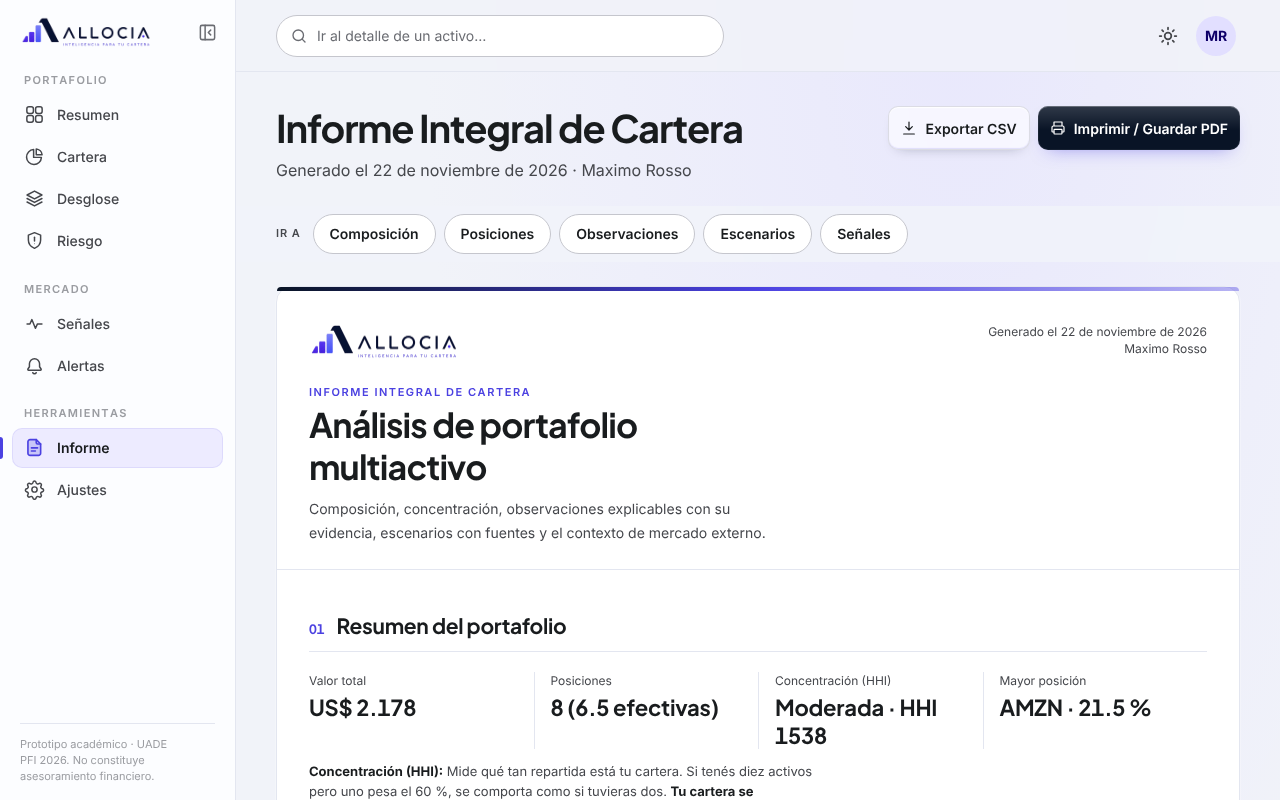
\includegraphics[width=0.82\textwidth]{figures/pantallas/web/a-08-informe.png}
	\caption{Capturas de mercados y alertas, y del informe de la cartera. Fuente: elaboración propia.}\label{fig:anx-alertas}
\end{figure}
\begin{figure}[ht]
	\centering
	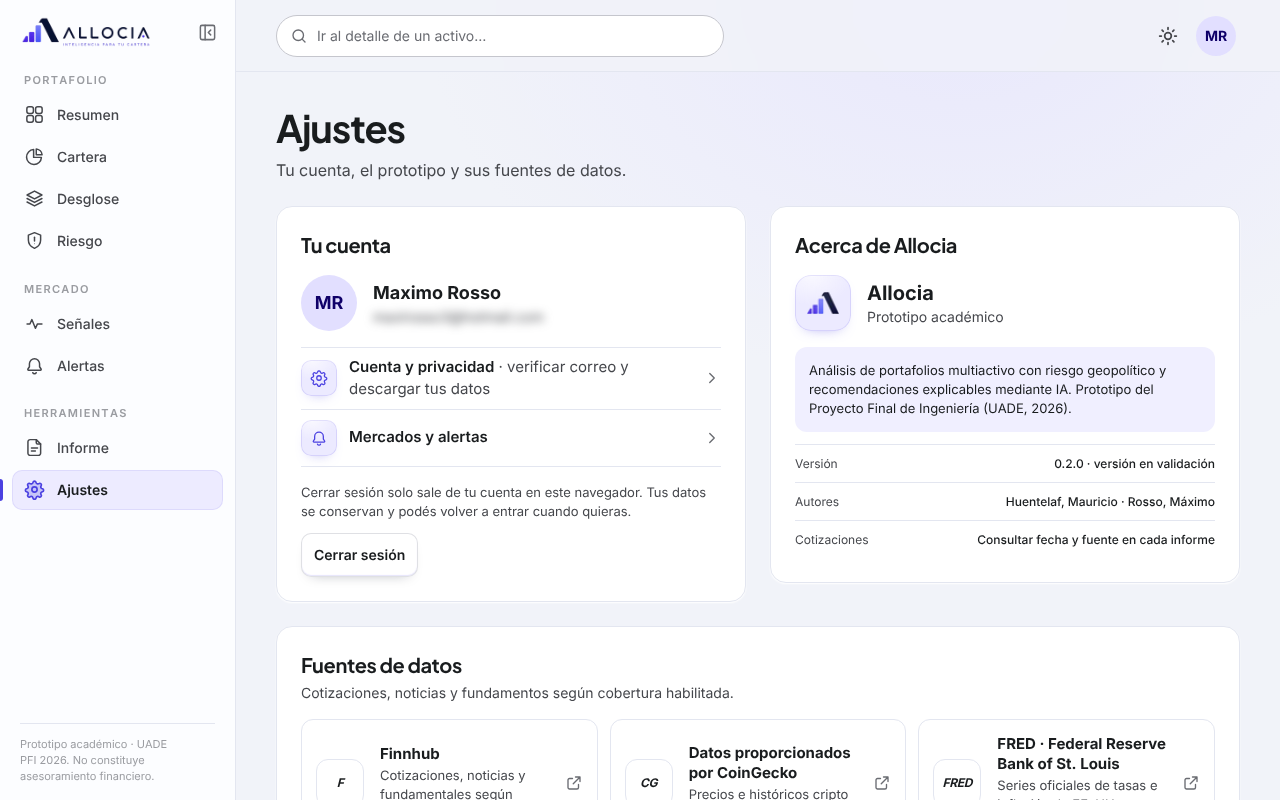
\includegraphics[width=0.82\textwidth]{figures/pantallas/web/a-09-ajustes.png}
	\caption{Captura de la pantalla de ajustes, con las fuentes de datos y el aviso del prototipo. Fuente: elaboración propia.}\label{fig:anx-ajustes}
\end{figure}

\section*{Wireframes del diseño original}
Los wireframes son anteriores a la implementación y tienen formato móvil. Cubren la bienvenida, el acceso y el registro (Figura~\ref{fig:wf-onboarding}), las secciones del diseño (Figuras~\ref{fig:wf-principales} y~\ref{fig:wf-senales}) y el desglose con el detalle por activo (Figura~\ref{fig:wf-detalle}). Alguna función que aparece en ellos, como la simulación de escenarios, se reemplazó durante la implementación por escenarios con fuentes (Subsección~\ref{sec:implementacion}).
\begin{figure}[ht]
	\centering
	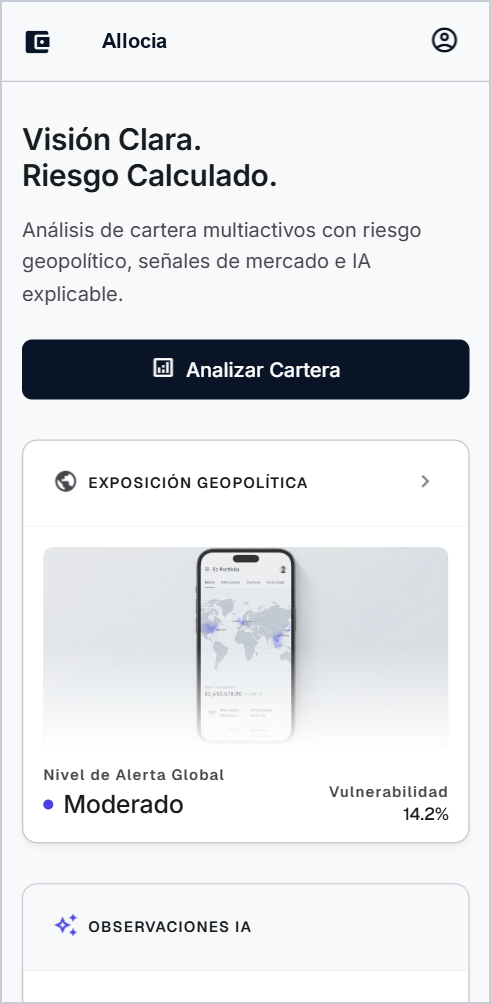
\includegraphics[height=9cm]{figures/wireframes/inicio.png}
	\hspace{0.35cm}
	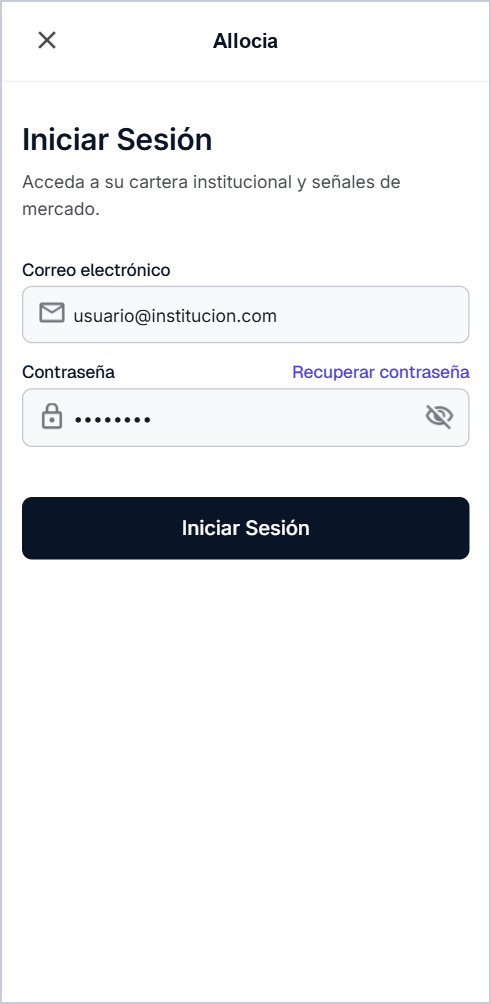
\includegraphics[height=9cm]{figures/wireframes/login.png}
	\hspace{0.35cm}
	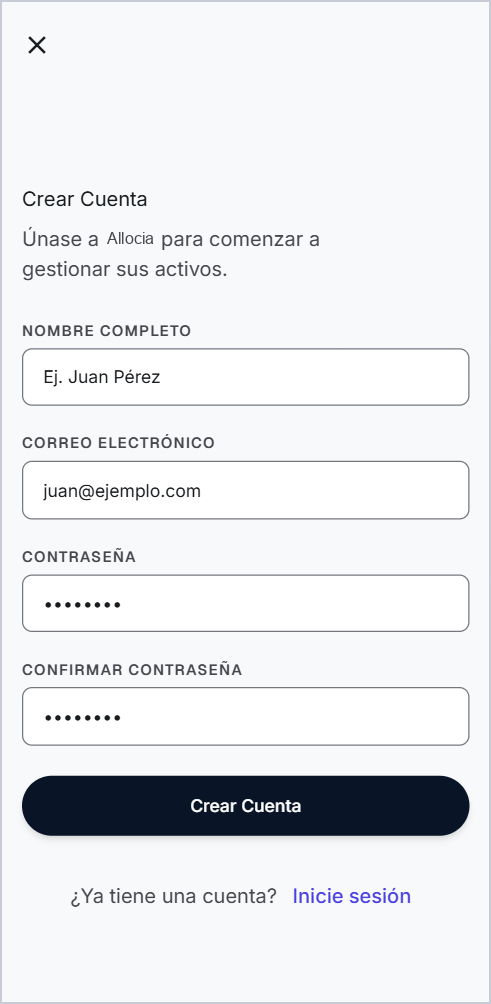
\includegraphics[height=9cm]{figures/wireframes/registro.png}
	\caption{Wireframes de bienvenida, inicio de sesión y registro (diseño de identidad). Fuente: elaboración propia.}
	\label{fig:wf-onboarding}
\end{figure}

\begin{figure}[ht]
	\centering
	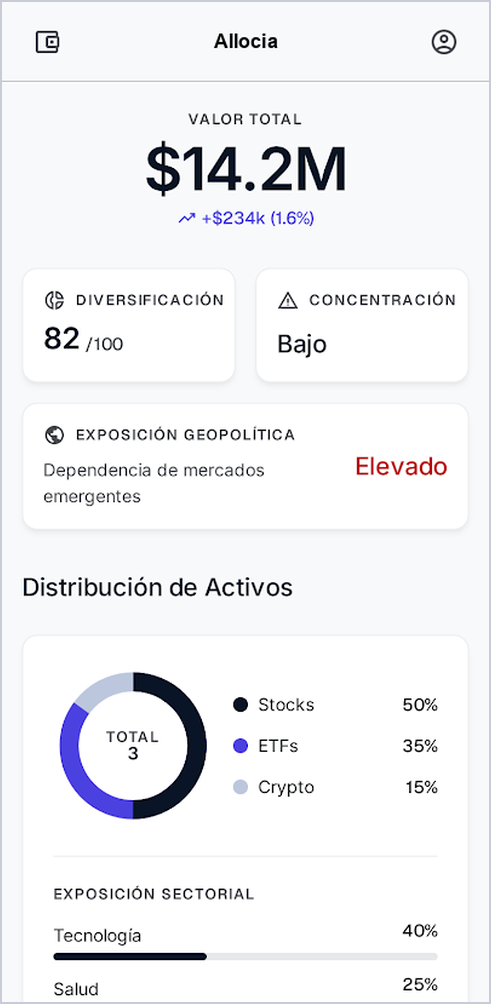
\includegraphics[height=9cm]{figures/wireframes/panel_principal.png}
	\hspace{0.35cm}
	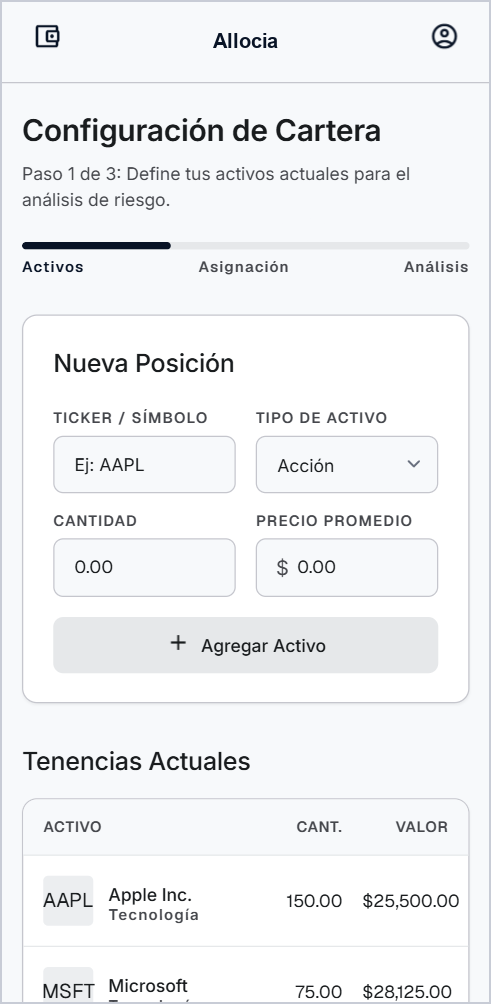
\includegraphics[height=9cm]{figures/wireframes/configuracion_cartera.png}
	\hspace{0.35cm}
	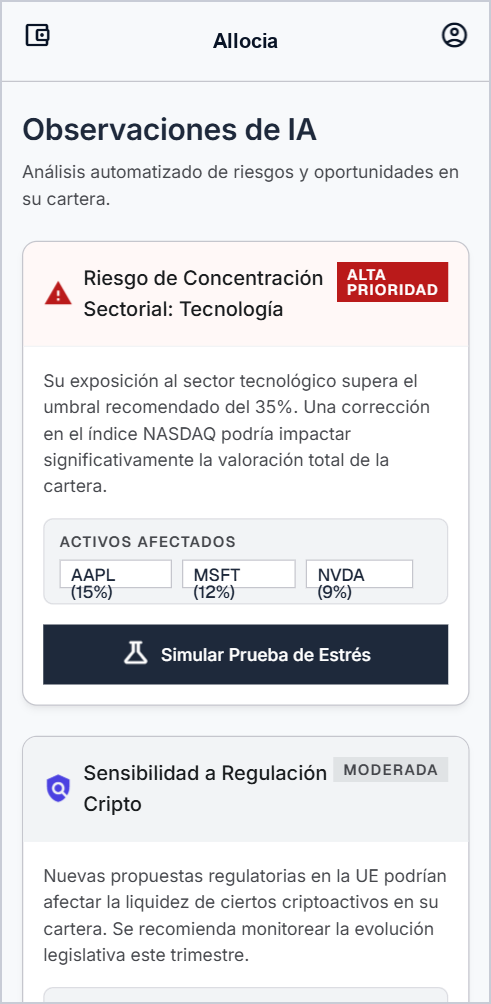
\includegraphics[height=9cm]{figures/wireframes/observaciones_ia.png}
	\caption{Wireframes de las secciones principales: panel de resumen, configuración de cartera y observaciones de IA. Fuente: elaboración propia.}
	\label{fig:wf-principales}
\end{figure}

\begin{figure}[ht]
	\centering
	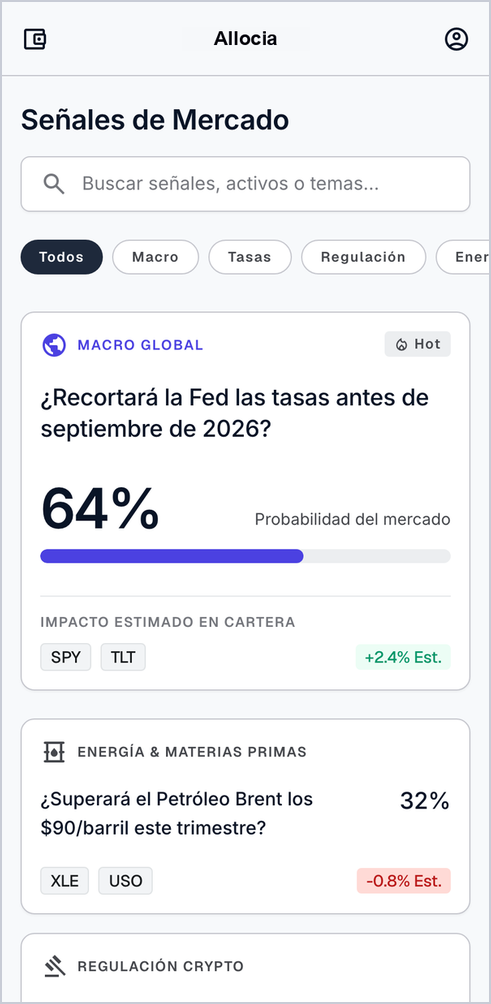
\includegraphics[height=9cm]{figures/wireframes/senales.png}
	\hspace{0.35cm}
	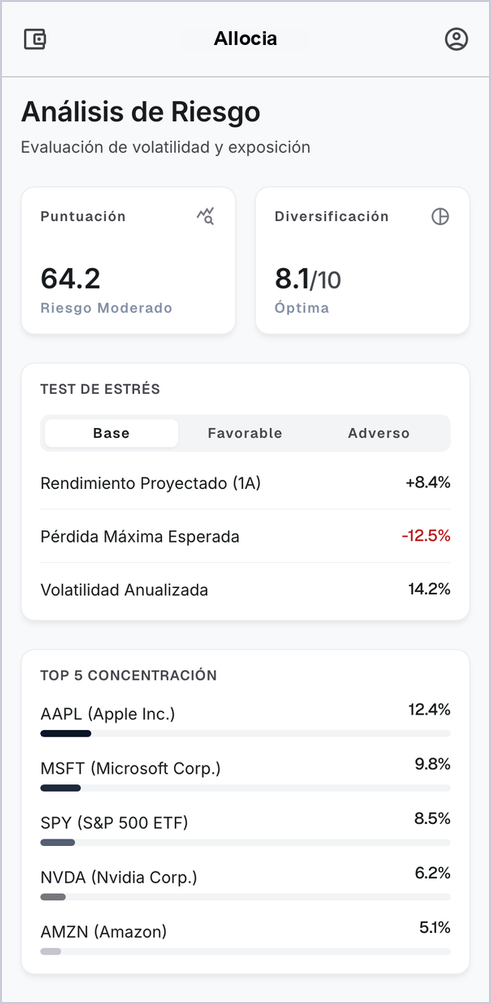
\includegraphics[height=9cm]{figures/wireframes/analisis_riesgo.png}
	\hspace{0.35cm}
	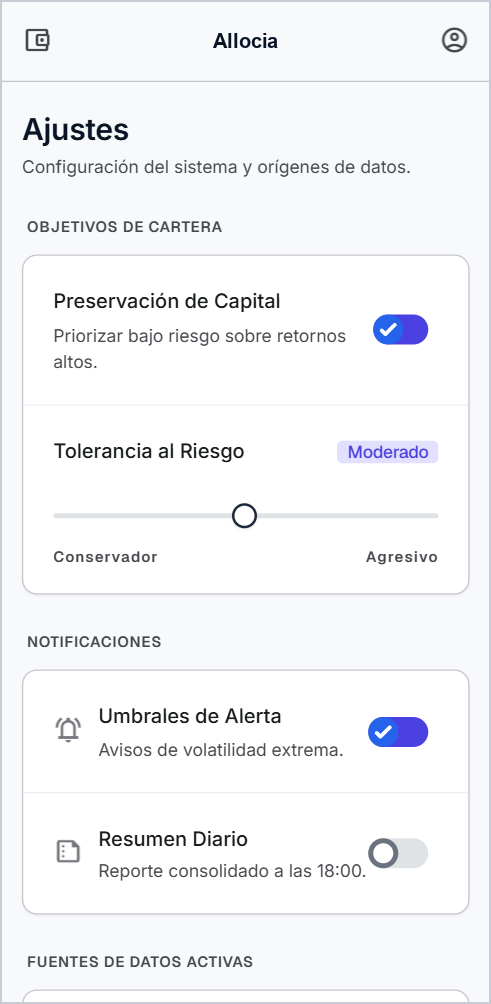
\includegraphics[height=9cm]{figures/wireframes/ajustes.png}
	\caption{Wireframes de señales de mercado, análisis de riesgo y ajustes. Fuente: elaboración propia.}
	\label{fig:wf-senales}
\end{figure}

\begin{figure}[ht]
	\centering
	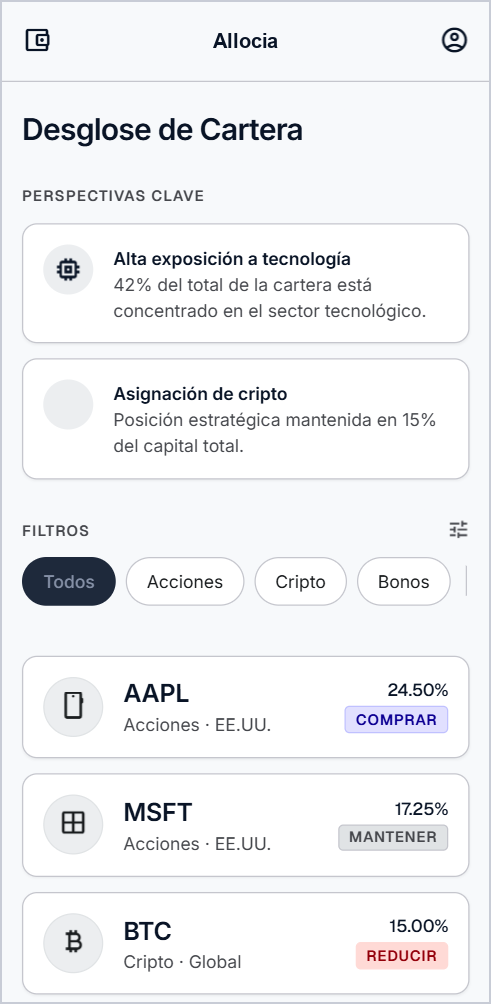
\includegraphics[height=9cm]{figures/wireframes/desglose.png}
	\hspace{0.35cm}
	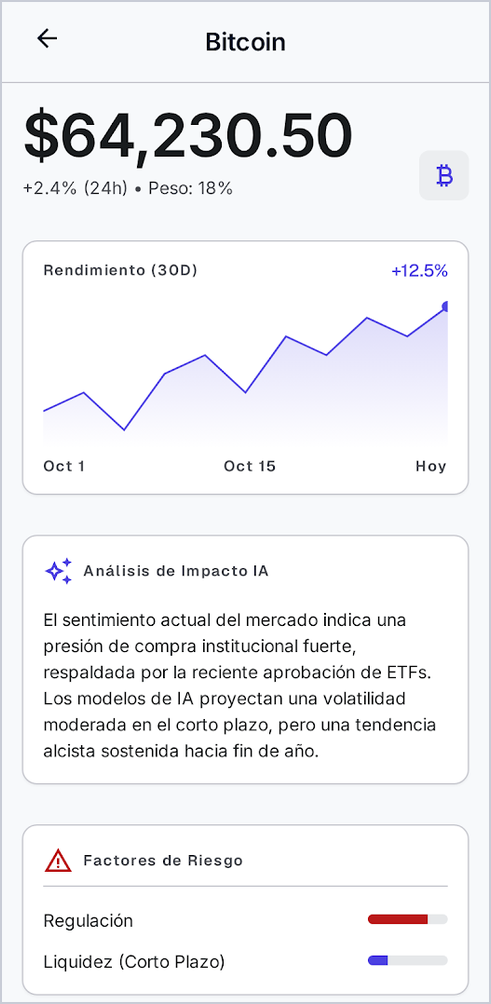
\includegraphics[height=9cm]{figures/wireframes/detalle.png}
	\caption{Wireframes de desglose de la cartera y detalle por activo. Fuente: elaboración propia.}
	\label{fig:wf-detalle}
\end{figure}

\section*{Privacidad y baja de cuenta en el diseño}
El diseño agrega, desde Ajustes, un acceso a la privacidad y a la eliminación de la cuenta. La Figura~\ref{fig:wf-privacidad} muestra el flujo que exigen RF9 y RF10, implementado y comprobado en el prototipo (Subsección~\ref{sec:pruebas-funcionales} y Subsubsección~\ref{sec:reverificacion-octubre13}); el esquema reproduce el diseño original. El aviso debe indicar responsable, finalidad, datos tratados, plazo de conservación y canal para ejercer derechos. La confirmación de baja debe explicar que se eliminan las posiciones y qué ocurre con las copias de seguridad según la política aplicable.
\begin{figure}[ht]\centering
\begin{tikzpicture}[box/.style={draw,rounded corners,text width=5.1cm,minimum height=5.5cm,align=left,inner sep=10pt,font=\small}]
\node[box,fill=blue!3] (a) {\textbf{Ajustes / Privacidad}\\[8pt]Datos de la cuenta.\\Finalidad del tratamiento.\\Conservación y derechos.\\Canal de contacto.\\[12pt]\fbox{Solicitar baja de cuenta}};
\node[box,fill=red!3,right=1cm of a] (b) {\textbf{Confirmar eliminación}\\[8pt]Cuenta y posiciones afectadas.\\Información sobre copias.\\Reautenticación.\\[12pt]\fbox{Cancelar}\\[8pt]\fbox{Confirmar eliminación}};
\draw[-{Stealth},thick] (a)--(b);
\end{tikzpicture}
\caption{Diseño del flujo de privacidad y baja. Fuente: elaboración propia.}\label{fig:wf-privacidad}
\end{figure}
            % Wireframes
\anexo{Encuesta: instrumento y resultados agregados}\label{annex:user-research}

Este anexo reproduce el cuestionario, las frecuencias agregadas de las preguntas cerradas y las respuestas a la pregunta abierta en que se apoya la Subsubsección~\ref{subsec:encuesta}. Las preguntas se transcriben tal como figuraban en el relevamiento, con sus redundancias incluidas.

\section*{Encuesta: formulario completo y respuestas}

La encuesta, titulada \textit{Encuesta sobre análisis y gestión de inversiones}, se administra con Google Forms y queda abierta del 24 de mayo al 14 de agosto de 2026; en ese período se registran 190 respuestas completas. A continuación se transcribe el formulario completo tal como lo vieron los encuestados. La Tabla~\ref{tab:encuesta-distribucion} presenta la distribución de respuestas de cada pregunta cerrada, la Tabla~\ref{tab:encuesta-temas} la codificación temática de la pregunta abierta y la Tabla~\ref{tab:encuesta-abierta} la transcripción de sus respuestas.

\subsection*{Formulario completo}

El formulario incluye opciones únicas, selecciones múltiples, escalas y una pregunta abierta.

\begin{enumerate}
    \item \textbf{Rango de edad.} Opción única: 18--24; 25--34; 35--44; 45+.
    \item \textbf{¿Cuál de estas situaciones te representa mejor?} Opción única: Invierto actualmente de forma activa; Invierto, pero hago seguimiento ocasional; No invierto actualmente, pero me interesa empezar; No invierto y no me interesa por ahora.
    \item \textbf{Tu nivel de conocimiento financiero.} Escala de 1 (muy bajo) a 5 (muy alto).
    \item \textbf{¿Qué tipos de activos tenés actualmente o te interesaría tener?} Selección múltiple: Acciones / CEDEARs; ETFs; Criptomonedas; Stablecoins / DeFi; Bonos / FCI / Plazo fijo; Dólar (MEP, CCL, físico); Otros / Ninguno todavía.
    \item \textbf{¿En cuántas plataformas distintas (brokers + exchanges) tenés activos o seguís inversiones?} Opción única: Ninguna todavía; 1; 2; 3; 4 o más.
    \item \textbf{¿Cómo hacés hoy el seguimiento de tu portafolio?} Opción única: Uso la app de cada plataforma por separado; Llevo un Excel / Google Sheets propio; Uso una app de tracking o portfolio management; Lo sigo de forma poco ordenada; No sigo un portafolio todavía.
    \item \textbf{¿Sentís que la información que necesitás para analizar tus inversiones está repartida entre muchas fuentes?} Escala de 1 (para nada) a 5 (totalmente).
    \item \textbf{¿Cuáles son tus principales dificultades al gestionar o analizar tu portafolio? (hasta 3)} Selección múltiple: Tener visión consolidada de todo; Saber si estoy bien diversificado; Entender mi exposición real (sector, región, moneda); Interpretar contexto macro y geopolítico; Seguir el mundo cripto / DeFi; Saber cuándo rebalancear; Falta de tiempo para investigar; No sé qué fuentes son confiables; Traducir mucha información en conclusiones claras.
    \item \textbf{¿Alguna vez te enteraste tarde de algo (noticia, evento) que habría cambiado una decisión de inversión?} Opción única: Sí, varias veces; Sí, alguna vez; No estoy seguro; No.
    \item \textbf{¿Conocés o usaste plataformas de prediction markets (por ejemplo, Polymarket)?} Opción única: Sí, las uso activamente; Sí, las conozco pero no las uso; No las conocía.
    \item \textbf{¿Te interesaría que una herramienta de análisis de portafolio incorpore señales basadas en probabilidades de eventos futuros (por ejemplo, tasas, inflación, elecciones o regulaciones)?} Escala de 1 (nada interesado) a 5 (muy interesado).
    \item \textbf{Si existiera una plataforma web que te permita cargar tu portafolio (acciones + ETFs + cripto) y te dé análisis integrado con contexto geopolítico y señales de mercado, ¿qué tan interesado estarías?} Escala de 1 (nada interesado) a 5 (muy interesado).
    \item \textbf{De estas funcionalidades, marcá las 3 más valiosas para vos.} Selección múltiple: Vista consolidada de todos mis activos; Análisis de diversificación y exposición real; Análisis fundamental básico de mis activos; Alertas sobre eventos geopolíticos relevantes para mi portafolio; Señales del ecosistema cripto / DeFi / prediction markets; Recomendaciones explicables (que muestren el por qué); Sugerencias de rebalanceo.
    \item \textbf{¿Qué tan importante te parece que una herramienta de IA explique por qué te muestra una observación o recomendación?} Escala de 1 (nada importante) a 5 (muy importante).
    \item \textbf{¿Usás o usaste alguna herramienta similar?} Opción única: Sí, la uso actualmente; La usé y la dejé; Las conozco pero no las uso; No conocía ninguna.
    \item \textbf{¿Qué sentís que le falta a las herramientas que usás hoy para analizar mejor tu portafolio?} Pregunta abierta.
    \item \textbf{¿Pagarías por una herramienta así?} Opción única: Sí, mensualmente; Solo si tiene versión gratuita con funciones pagas; Solo si es 100\,\% gratis; No la usaría.
\end{enumerate}

\subsection*{Distribución de respuestas}

Los porcentajes toman N=190 como denominador; en las preguntas de selección múltiple pueden sumar más de 100\,\%, y las pequeñas diferencias en las sumas se deben al redondeo. Fuente: elaboración propia sobre las frecuencias documentadas en el relevamiento.

{
\small
\singlespacing
\setlength{\tabcolsep}{5pt}
\renewcommand{\arraystretch}{1.15}
\begin{longtable}{p{9.3cm} r r}
	\caption{Distribución de respuestas (N=190). Fuente: elaboración propia.}
	\label{tab:encuesta-distribucion}\\
	\hline
	\textbf{Pregunta / Opción} & \textbf{n} & \textbf{\%} \\
	\hline
	\endfirsthead
	\hline
	\textbf{Pregunta / Opción} & \textbf{n} & \textbf{\%} \\
	\hline
	\endhead
	\hline
	\endfoot
	\multicolumn{3}{l}{\textbf{1. Rango de edad}} \\
	\quad 18--24 & 58 & 30,5 \\
	\quad 25--34 & 77 & 40,5 \\
	\quad 35--44 & 37 & 19,5 \\
	\quad 45+ & 18 & 9,5 \\
	\multicolumn{3}{l}{\textbf{2. Situación frente a la inversión}} \\
	\quad Invierto actualmente de forma activa & 85 & 44,7 \\
	\quad Invierto, pero hago seguimiento ocasional & 57 & 30,0 \\
	\quad No invierto actualmente, pero me interesa empezar & 36 & 18,9 \\
	\quad No invierto y no me interesa por ahora & 12 & 6,3 \\
	\multicolumn{3}{l}{\textbf{3. Nivel de conocimiento financiero (media: 3,17)}} \\
	\quad 1 & 17 & 8,9 \\
	\quad 2 & 33 & 17,4 \\
	\quad 3 & 60 & 31,6 \\
	\quad 4 & 61 & 32,1 \\
	\quad 5 & 19 & 10,0 \\
	\multicolumn{3}{l}{\textbf{4. Tipos de activos que tiene o le interesaría tener (múltiple)}} \\
	\quad Acciones / CEDEARs & 129 & 67,9 \\
	\quad ETFs & 105 & 55,3 \\
	\quad Dólar (MEP, CCL, físico) & 103 & 54,2 \\
	\quad Bonos / FCI / Plazo fijo & 90 & 47,4 \\
	\quad Criptomonedas & 90 & 47,4 \\
	\quad Stablecoins / DeFi & 49 & 25,8 \\
	\quad Otros / Ninguno todavía & 13 & 6,8 \\
	\multicolumn{3}{l}{\textbf{5. Cantidad de plataformas (brokers + exchanges)}} \\
	\quad Ninguna todavía & 24 & 12,6 \\
	\quad 1 & 24 & 12,6 \\
	\quad 2 & 44 & 23,2 \\
	\quad 3 & 37 & 19,5 \\
	\quad 4 o más & 61 & 32,1 \\
	\multicolumn{3}{l}{\textbf{6. Forma de seguimiento del portafolio}} \\
	\quad Uso la app de cada plataforma por separado & 58 & 30,5 \\
	\quad Llevo un Excel / Google Sheets propio & 41 & 21,6 \\
	\quad No sigo un portafolio todavía & 41 & 21,6 \\
	\quad Uso una app de tracking o portfolio management & 28 & 14,7 \\
	\quad Lo sigo de forma poco ordenada & 22 & 11,6 \\
	\multicolumn{3}{l}{\textbf{7. Percepción de información repartida entre muchas fuentes (media: 3,51)}} \\
	\quad 1 & 13 & 6,8 \\
	\quad 2 & 30 & 15,8 \\
	\quad 3 & 38 & 20,0 \\
	\quad 4 & 66 & 34,7 \\
	\quad 5 & 43 & 22,6 \\
	\multicolumn{3}{l}{\textbf{8. Principales dificultades (múltiple, hasta 3)}} \\
	\quad Tener visión consolidada de todo & 75 & 39,5 \\
	\quad Falta de tiempo para investigar & 68 & 35,8 \\
	\quad Saber si estoy bien diversificado & 60 & 31,6 \\
	\quad Seguir el mundo cripto / DeFi & 52 & 27,4 \\
	\quad Entender mi exposición real (sector, región, moneda) & 51 & 26,8 \\
	\quad Traducir mucha información en conclusiones claras & 50 & 26,3 \\
	\quad Interpretar contexto macro y geopolítico & 49 & 25,8 \\
	\quad No sé qué fuentes son confiables & 45 & 23,7 \\
	\quad Saber cuándo rebalancear & 38 & 20,0 \\
	\multicolumn{3}{l}{\textbf{9. Se enteró tarde de una noticia o evento relevante}} \\
	\quad Sí, alguna vez & 75 & 39,5 \\
	\quad Sí, varias veces & 56 & 29,5 \\
	\quad No estoy seguro & 36 & 18,9 \\
	\quad No & 23 & 12,1 \\
	\multicolumn{3}{l}{\textbf{10. Conocimiento de prediction markets}} \\
	\quad No las conocía & 103 & 54,2 \\
	\quad Sí, las conozco pero no las uso & 71 & 37,4 \\
	\quad Sí, las uso activamente & 16 & 8,4 \\
	\multicolumn{3}{l}{\textbf{11. Interés en señales basadas en probabilidades de eventos (media: 3,53)}} \\
	\quad 1 & 11 & 5,8 \\
	\quad 2 & 30 & 15,8 \\
	\quad 3 & 45 & 23,7 \\
	\quad 4 & 55 & 28,9 \\
	\quad 5 & 49 & 25,8 \\
	\multicolumn{3}{l}{\textbf{12. Interés en la plataforma propuesta (media: 3,92)}} \\
	\quad 1 & 7 & 3,7 \\
	\quad 2 & 13 & 6,8 \\
	\quad 3 & 32 & 16,8 \\
	\quad 4 & 74 & 38,9 \\
	\quad 5 & 64 & 33,7 \\
	\multicolumn{3}{l}{\textbf{13. Funcionalidades más valiosas (múltiple, hasta 3)}} \\
	\quad Vista consolidada de todos mis activos & 116 & 61,1 \\
	\quad Análisis de diversificación y exposición real & 89 & 46,8 \\
	\quad Recomendaciones explicables (que muestren el por qué) & 88 & 46,3 \\
	\quad Alertas sobre eventos geopolíticos relevantes & 78 & 41,1 \\
	\quad Sugerencias de rebalanceo & 72 & 37,9 \\
	\quad Análisis fundamental básico de mis activos & 64 & 33,7 \\
	\quad Señales del ecosistema cripto / DeFi / prediction markets & 62 & 32,6 \\
	\multicolumn{3}{l}{\textbf{14. Importancia de la explicabilidad en herramientas de IA (media: 3,64)}} \\
	\quad 1 & 9 & 4,7 \\
	\quad 2 & 26 & 13,7 \\
	\quad 3 & 41 & 21,6 \\
	\quad 4 & 62 & 32,6 \\
	\quad 5 & 52 & 27,4 \\
	\multicolumn{3}{l}{\textbf{15. Uso de herramientas similares}} \\
	\quad No conocía ninguna & 81 & 42,6 \\
	\quad Las conozco pero no las uso & 43 & 22,6 \\
	\quad La usé y la dejé & 42 & 22,1 \\
	\quad Sí, la uso actualmente & 24 & 12,6 \\
	\multicolumn{3}{l}{\textbf{17. Disposición a pagar}} \\
	\quad Solo si tiene versión gratuita con funciones pagas & 95 & 50,0 \\
	\quad Sí, mensualmente & 49 & 25,8 \\
	\quad Solo si es 100\,\% gratis & 30 & 15,8 \\
	\quad No la usaría & 16 & 8,4 \\
\end{longtable}
}

\subsection*{Respuestas a la pregunta abierta}

La pregunta 16 recibió 190 respuestas, de las cuales 27 no aportan contenido: un guion, un punto o expresiones como \enquote{no sé} y \enquote{no uso}. Las 163 restantes se codificaron por tema con el programa \texttt{scripts/codificar\_respuestas\_abiertas.py} del repositorio del Proyecto, que asigna cada tema según las expresiones presentes en el texto; la asignación se revisó respuesta por respuesta, y una respuesta puede corresponder a más de un tema. La Tabla~\ref{tab:encuesta-temas} presenta las frecuencias, con porcentajes sobre las 163 respuestas sustantivas. La Tabla~\ref{tab:encuesta-abierta} transcribe las 190 respuestas en el orden en que se registraron, sin corregir ortografía ni redacción; algunos textos se repiten de forma idéntica o con variaciones mínimas.

\begin{table}[ht]
\centering\small\renewcommand{\arraystretch}{1.15}
\caption{Temas de las respuestas a la pregunta abierta (163 respuestas sustantivas). Fuente: elaboración propia.}\label{tab:encuesta-temas}
\begin{tabular}{>{\raggedright\arraybackslash}p{10.2cm}rr}\hline
\textbf{Tema} & \textbf{n} & \textbf{\%}\\\hline
Contexto argentino: inflación, tipo de cambio e instrumentos locales & 46 & 28,2 \\
Consolidación e integración entre plataformas & 39 & 23,9 \\
Noticias, alertas y efecto del contexto sobre la cartera & 34 & 20,9 \\
Carga y actualización automáticas & 23 & 14,1 \\
Lenguaje accesible y facilidad de uso & 18 & 11,0 \\
Exposición real, diversificación y composición de fondos & 18 & 11,0 \\
Criptoactivos, DeFi y mercados de predicción & 18 & 11,0 \\
Explicación y fundamento de las observaciones & 14 & 8,6 \\
Falta de tiempo para seguir y procesar la información & 10 & 6,1 \\
Otros temas & 6 & 3,7 \\
\hline

\end{tabular}
\end{table}
\FloatBarrier

{
\footnotesize
\singlespacing
\setlength{\tabcolsep}{5pt}
\renewcommand{\arraystretch}{1.1}
\begin{longtable}{r >{\raggedright\arraybackslash}p{13.6cm}}
	\caption{Respuestas a la pregunta abierta, en orden de registro (N=190). Fuente: elaboración propia.}
	\label{tab:encuesta-abierta}\\
	\hline
	\textbf{N.º} & \textbf{Respuesta} \\
	\hline
	\endfirsthead
	\hline
	\textbf{N.º} & \textbf{Respuesta} \\
	\hline
	\endhead
	\hline
	\endfoot
	1 & - \\
2 & No lo sé \\
3 & No uso \\
4 & No conozco ninguna \\
5 & Que se agreguen automáticamente las operaciones que hago en cualquiera de mis cuentas. No tener que cargarlas manualmente. Por otro lado, jamás confiaría en las recomendaciones de la IA, deben tener sustento en algún reserach que ya exista, incluir fuentes, views de equipos de research de distintos brokers puede ser interesante \\
6 & Conocer la ganancia real. En Argentina muchas de las inversiones son en pesos y debido a la inflación es complicado saber si vas ganando o perdiendo. Con los CEDEARs también es un problema ya que su valor está ajustado con el dólar CCL dificultando calcular la ganancia de la inversión \\
7 & Aparte de los analyst ratings, información de porque creen que el activo subirá o bajará. Si tengo una IA que me ayude con esto. Sería increíble \\
8 & Mejor analisis de que compre y que vendi para saber la ganancia real de mi portafolio \\
9 & Análisis de los componentes de cada ETF/MF para conocer exposición real \\
10 & Contexto inflacionario y geopolitico \\
11 & No uso ninguna herramienta pero el proyecto me parece una buena idea. \\
12 & personalización y el conocimiento profundo del negocio \\
13 & Poder tener todo en una sola plataforma \\
14 & Hacerse mas visibles. \\
15 & Resumen de noticias relacionadas a mis inversiones. \\
16 & Recomendaciones explicables \\
17 & Integración con otras plataformas \\
18 & No lo sé \\
19 & - \\
20 & Mas claridad y fácil utilización \\
21 & No conozco mucho de inversión \\
22 & Analisis \\
23 & Compra venta mas facil, mejor ux \\
24 & - \\
25 & confidencialidad \\
26 & Que puedan comparar exposición real \\
27 & No conozco ninguna \\
28 & No aplica \\
29 & Ni idea \\
30 & Tenes todo consolidado en un lugar y a partir de ahí tomar decisiones. \\
31 & . \\
32 & \_ \\
33 & Me cuesta tener todo junto en un solo lugar. Uso varias apps y pierdo tiempo consolidando datos manualmente cada semana. \\
34 & facilidad de conectar con mi portafolio actual \\
35 & No uso ese tipo de herramientas \\
36 & el problema es que tengo todo en pesos y no se bien como estoy expuesto al dolar en total. \\
37 & no encuentro nada que ande bien para el mercado argentino, todo esta pensado para afuera \\
38 & tiempo. no tengo tiempo de analizar todo yo solo. \\
39 & no encuentro nada que ande bien para el mercado argentino, todo esta pensado para afuera \\
40 & tmb me pasa que me entero de noticias importantes cuando ya es tarde lamentablemente \\
41 & cada vez que pasa algo macro tardo horas en entender si me afecta a mi o no. \\
42 & osea tengo cripto en binance y cedears en balanz y no hay forma de unirlo todo \\
43 & sigo tips de un grupo de telegram. se que no es lo ideal pero no encontre algo mejor. \\
44 & osea tengo cripto en binance y cedears en balanz y no hay forma de unirlo todo \\
45 & Necesito poder ver mi exposicion real por moneda, sector y region en un solo lugar. Hoy eso requiere mucho trabajo manual. \\
46 & el problema es que tengo todo en pesos y no se bien como estoy expuesto al dolar en total. \\
47 & las herraminetas que probe son muy tecnicas, necesito algo mas acccesible para mi nivel \\
48 & perdí plata por no enterarme a tiempo de una noticia, me hubiera venido bien una alerta \\
49 & que explique las cosas en criollo y no en terminos tecnicos. \\
50 & me falta una vista que me diga: esto es lo que tenes, esto es lo que rinde, esto es lo que riesgo. \\
51 & Lo que mas valoro es la explicabilidad. No alcanza con que me digan que hacer, necesito entender el razonamiento detras. \\
52 & Uso varias billeteras y plataformas y es un caos cuando quiero saer cuánto tengo \\
53 & Integración con IOL y Balanz como mínimo. \\
54 & No aplica \\
55 & tengo todo en DeFi y no hay ninguna app que integre eso con mis CEDEARs en Balanz. \\
56 & Mi problema es que invierto pero no entiendo bien lo que hago necesito más ayuda \\
57 & Análisis de la exposición real considerando los subyacentes de los CEDEARs y ETFs, no solo el valor nominal de las posiciones. \\
58 & Tengo cuenta en Balanz en IOL y en Lemon y cada uno me muestra sus números pero nunca veo el cuadro completo \\
59 & Me pasa que tengo FCI, CEDEARs y dólar MEP en distintos lados y nunca veo el total. \\
60 & Me falta una herramienta que integre el análisis fundamental con el contexto macroeconómico de forma automática y comprensible. \\
61 & Lo que más falta en el mercado argentino es una herramienta que trate las CEDEARs como lo que son: exposición a acciones extranjeras con riesgo cambiario local. \\
62 & sin comentarios \\
63 & Me cuesta saber si estoy bien diversificado o si en realidad estoy súper concentrado en algo. \\
64 & Alertas de noticias relevantes para mis posiciones. \\
65 & Automatizar la carga de operaciones. \\
66 & Que no sea tan técnico. \\
67 & No sé \\
68 & Visión consolidada de todo, eso es lo que falta. \\
69 & El análisis de liquidez de mis posiciones es algo que nunca contemplo bien. No sé cuánto tiempo me llevaría salir de cada activo si necesitara el dinero. \\
70 & Lo de la ganancia real en Argentina es muy complicado por la inflación y el tipo de cambio. \\
71 & Estaría bueno que me sugiera qué hacer cuando algo en el mercado cambia mucho. \\
72 & no entiendo nada de macro pero igual invierto, necesito que alguien me explique \\
73 & Uso varias billeteras y plataformas y es un caos cuando quiero saer cuánto tengo \\
74 & Lo que falta es algo que integre on-chain con off-chain en un solo dashboard. \\
75 & no se me ocurre nada \\
76 & El tema del tipo de cambio en Argentina complica todo. Uno no sabe bien si gano o no \\
77 & Alertas en tiempo real. \\
78 & no uso herramientas \\
79 & Me gustaría entender mejor los ETFs que tengo, qué hay adentro de cada uno. \\
80 & Me fala contexto macro. Sé que sube o baja pero no entiendo por q impacta en mí \\
81 & Me falta una vista que me diga: esto es lo que tenés, esto es lo que rinde, esto es lo que arriesgás. \\
82 & El seguimiento del ecosistema DeFi en conjunto con activos tradicionales es algo que ninguna herramienta local ofrece de forma integrada. \\
83 & Re complicado seguir todo junto. Necesito algo que lo haga automático ya \\
84 & Lo que más me molesta es que cuando quiero saber cuánto tengo en total tengo que abrir todo y calcularlo a mano \\
85 & Uso excel pero no tengo precios en tiempo real. \\
86 & Que me diga cuánto tengo en dólares reales, no nominales. \\
87 & Lo que más me falta es contexto. No solo precios sino por qué están subiendo o bajando. \\
88 & Mejor UX en general. \\
89 & Capaz me falta una herramienta que lo explique más simple, soy re principiante todavía \\
90 & Que me diga cuánto gané de verdad descontando inflación, eso es lo q más necesito \\
91 & Cada vez que suben las tasas no entiendo si eso me conviene o no, es medio confuso todo \\
92 & Tiempo y claridad. Eso es lo que más me falta para tomar mejores decisiones de inversión. \\
93 & Lo que más me molesta es no tener alertas cuando hay noticias que me pueden afectar. \\
94 & Lo que busco es algo que me traduzca la macro global en impacto concreto en mi portafolio. \\
95 & Igual lo sigo bastante poco la verdad, me falta tiempo y ganas de organizar todo \\
96 & Nada que sirva para el contexto argentino. \\
97 & Uso un excel que hice yo pero es un quilombo actualizarlo. Necesito algo automático. \\
98 & Todo muy fragmentado, abro 4 apps distintas y nunca veo el total real \\
99 & Información contextualizada para Argentina. \\
100 & N/A \\
101 & El excel me quedó chico pero no encontré nada mejor para el mercado local \\
102 & Probé apps pero ninguna entiende el mercado local. \\
103 & Integración con IOL y Balanz como mínimo. \\
104 & No entiendo bien mi exposición real, creo q tengo más riesgo del que pienso \\
105 & Poder ver todo en un solo lugar. \\
106 & Tengo un excel con 8 pestañas y igual no me alcanza. \\
107 & Tmbn me pasa que veo una noticia y no sé si me afecta a mí o no, es medio frustrante \\
108 & no lo sé \\
109 & ninguna \\
110 & Perdí plata por no enterarme a tiempo de una noticia, me hubiera venido bien una alerta \\
111 & Las herramientas existentes no contemplan el contexto argentino: inflación, tipo de cambio, riesgo país. Eso hace que el análisis quede incompleto. \\
112 & Me pasa seguido que veo algo en Twitter y no sé si es relevante para mis posiciones o es solo ruido y termino no haciendo nada \\
113 & Análisis de riesgo sencillo de entender. \\
114 & Me gustaría saber cuándo una noticia geopolítica me impacta directamente. \\
115 & Quería empezar a invertir pero no sé ni por dónde, todas las apps son muy confusas \\
116 & nose \\
117 & El análisis de ETFs debería incluir la composición interna para conocer la exposición real por sector y región, no solo el precio del ETF. \\
118 & Que las operaciones se carguen solas, cargarlas a mano es lo que más abandono. \\
119 & El problema es que la info está en todos lados y no tengo tiempo de procesarla toda y sacar una conclusión clara \\
120 & Lo que más valoro es la explicabilidad. No alcanza con que me digan qué hacer, necesito entender el razonamiento detrás. \\
121 & Lo de las CEDEARs es re complicado porque no sé si ganás en dólares de verdad o es todo dólar CCL \\
122 & La visualización de la exposición por moneda es algo que ninguna herramienta local ofrece de forma clara y automática. \\
123 & La idea de tener todo integrado con alertas me parece lo más útil de todo lo que mencionan. \\
124 & el problema es que tengo todo en pesos y no sé bien cómo estoy expuesto al dólar en total. \\
125 & Me cuesta mucho entender cuánto de mi portafolio está dolarizado de verdad. \\
126 & Cuando veo que el dólar se mueve mucho no sé si mis inversiones me cubren o estoy perdiendo plata real \\
127 & nada \\
128 & Tengo un FCI en Galicia y CEDEARs en IOL y dólares en Brubank y es imposible ver todo junto sin abrir tres apps \\
129 & No entiendo por qué ninguna app integra CEDEARs con cripto con FCI es como si los brokers no quisieran que vieras todo junto \\
130 & Me gustaría poder ver mi ganancia ajustada por inflación, no solo en pesos nominales. \\
131 & Ni idea \\
132 & El contexto argentino es muy específico y las apps gringas no lo contemplan para nada. \\
133 & No encuntro nada que funcione para el mercado local, todo está pensado para afuera \\
134 & Que integre cripto con lo tradicional. Eso básicamente. \\
135 & Usé Personal Portfolio en su momento pero no contemplaba el mercado argentino y lo dejé. \\
136 & El principal problema es la fragmentación. Tengo activos en distintas plataformas y no hay forma de ver el total consolidado sin hacerlo manualmente. \\
137 & Que muestre rendimientos ajustados por inflación y riesgo país. \\
138 & Se me va todo el finde actualizando el excel, re pajero eso \\
139 & Tmb me pasa que me entero de noticias importantes cuando ya es tarde lamentablemente \\
140 & Cuando sale una noticia macro siempre me pregunto si me afecta, y me lleva horas entenderlo. \\
141 & Cuando ocurren eventos geopolíticos relevantes no tengo forma de saber rápidamente cuáles de mis posiciones pueden verse afectadas. \\
142 & Me interesaría poder comparar el rendimiento de mi portafolio contra benchmarks relevantes para el mercado argentino, no solo el S\&P. \\
143 & Las herraminetas que probé son muy técnicas, necesito algo más accesible para mi nivel \\
144 & Qué molesto tener que ir app por app para ver cómo estoy. Qué paja \\
145 & La verdad no tengo ni idea de cuándo rebalancear, lo hago bastante rapido \\
146 & Probé Bloomberg y otras apps y nada funciona bien para el mercado argentino hay que adaptar todo a mano \\
147 & Cargo todo a mano y siempre lo termino abandonando. \\
148 & Que tenga en cuenta la inflación argentina. \\
149 & Que expliquen qué hay adentro de cada CEDEAR, no solo el precio. \\
150 & Me cueta mucho encontrar info confiable, hay mucho influencer dando consejos sin saber \\
151 & El seguimiento de prediction markets no está integrado en ningún análisis de portafolio serio que yo conozca. \\
152 & Lo que necesito es algo que me diga en qué estoy invertido de verdad sector moneda riesgo todo junto \\
153 & Me cansé de los grupos de Telegram con tips, necesito algo más serio pero que se entienda \\
154 & Re útil sería una cosa que te avise cuando algo importante pasa y te diga si te afecta o no \\
155 & Lo de los prediction markets es interesante pero nadie lo integra con el portafolio tradicional. \\
156 & Recomendaciones con fundamento, no solo ''comprá esto''. \\
157 & Seguir el ecosistema cripto requiere como 5 apps distintas y sigue siendo incompleto. \\
158 & No encuentro nada que ande bien para el mercado argentino, todo está pensado para afuera \\
159 & Una cosa que valoro mucho es que me expliquen el razonamiento, no solo la recomendación. \\
160 & Que explique en criollo y no en términos técnicos. \\
161 & Me muevo mucho entre chains y es imposible seguir todo con una sola herramienta. \\
162 & Me gustaría integrar mi cuenta de Lemon con lo q tengo en IOL Investor Pro \\
163 & El yield farming lo trackeo a mano, no encontré nada automático. \\
164 & La falta de integración entre plataformas es el principal cuello de botella. Debería poder conectar mis cuentas de Balanz, IOL y Binance en un solo lugar. \\
165 & No sé cuánto de lo que gano es real y cuánto es inflación. \\
166 & Sigo un grupo de Telegram. No es lo ideal pero no encontré algo mejor. \\
167 & Igual sigo todo por Twitter más que por las apps, no sé si es lo mejor jaja \\
168 & Cada semana hago el mismo ritual de exportar datos de cada plataforma pegarlo en el excel y calcular el total es una pérdida de tiempo enorme \\
169 & Me gustaría una herramienta que contextualice cada evento macroeconómico en función de mi portafolio específico, no de forma genérica. \\
170 & Abrí cuenta en tres brokers y ahora no sé ni cuánto tengo en total \\
171 & Cada vez que leo noticias de economía argentina no sé si actuar o quedarme quieto porque no entiendo bien el impacto \\
172 & Necesito poder distinguir entre ganancia nominal y ganancia real. Hoy todo se mezcla. \\
173 & Probé Delta y Monarch y nada, ninguna soporta CEDEARs bien \\
174 & La mayoría de portfolio trackers no soportan tokens en Polygon o Arbitrum, es frustrante. \\
175 & Cada vez que pasa algo macro tardo horas en entender si me afecta a mí o no. \\
176 & Me pasa que leo cosas contradictorias en distintos medios y no sé a quién creerle para tomar decisiones \\
177 & Ojalá sincronización con Mercado Pago y Belo tmbn, ahí tengo plata parada \\
178 & Lo que más me cuesta es saber cuándo y cómo rebalancear. Nadie te lo explica bien. \\
179 & Me custa consolidar todo. Uso tres apps y ninguna se conecta con la otra \\
180 & El mayor problema es k todo está separado y no hay forma de verlo junto fácilmente \\
181 & Las recomendaciones que encuentro en internet son genéricas. Necesito algo que analice mi portafolio específico y me sugiera acciones concretas. \\
182 & No sé. Creo que con ver todo junto ya me cambia la vida. \\
183 & Lo que más me interesa es poder medir mi rendimiento real ajustado por inflación y tipo de cambio. Hoy eso requiere cálculos manuales muy tediosos. \\
184 & Me gustaría que me digan si estoy bien o mal y por qué no solo mostrarme números sin explicación \\
185 & El onboarding de casi todas las apps de inversión es un asco, muy técnico para alguien que empieza \\
186 & Necesito poder ver mi exposición real por moneda, sector y región en un solo lugar. Hoy eso requiere mucho trabajo manual. \\
187 & Sería muy útil poder simular escenarios: qué pasa con mi portafolio si el dólar sube un 30\% o si baja el riesgo país. \\
188 & Necesito algo que me muestre todo junto en un solo lugar y que se actualice solo sin que yo tenga que hacer nada \\
189 & Consolidación automática sin cargar nada a mano. \\
190 & Valoro mucho la transparencia en las recomendaciones. Si una IA me sugiere algo, necesito ver las fuentes y el razonamiento antes de actuar. \\

\end{longtable}
}
         % Encuesta
\anexo{Entrevistas: guía y perfiles}\label{annex:entrevistas}

Este anexo reúne la guía de entrevista y los perfiles de los tres participantes. Las transcripciones completas de las conversaciones, mantenidas el 22 de octubre de 2026 por videollamada, figuran en los Anexos~\ref{annex:entrevista-tadeo}, \ref{annex:entrevista-fabricio} y~\ref{annex:entrevista-octavio}. Cada registro consigna fecha, hora de inicio, entrevistador y duración. Las transcripciones son automáticas y se reproducen con una edición mínima: se corrigen entre corchetes los errores evidentes del reconocimiento de voz (por ejemplo, el broker Balanz transcripto como \enquote{Balance}) y, en la tercera, se suprimen las muletillas de inicio de frase sin alterar el contenido. Al inicio de cada conversación el entrevistador informa que las respuestas se usan para el Proyecto, lo que consta en la propia transcripción.

\section*{Guía utilizada}
La guía organiza la conversación en cinco ejes y se transcribe tal como se aplicó.
\begin{enumerate}
\item ¿Cómo es hoy tu manera de seguir y analizar tus inversiones? ¿Qué herramientas, apps o planillas usás y cómo las combinás?
\item Cuando tenés activos de distinto tipo (por ejemplo, acciones, ETFs y criptomonedas), ¿tus inversiones están todas en un mismo lugar o repartidas en varias apps o cuentas?
\item La última vez que tomaste una decisión de comprar, vender o reacomodar tu cartera, ¿en qué información te basaste y qué te hubiera gustado tener y no tenías?
\item ¿Alguna vez una app o plataforma te dio una alerta, sugerencia o recomendación sobre tus inversiones? ¿Entendiste por qué te la daba y qué tanto confiaste en ella?
\item Si pudieras pedirle cualquier cosa a una herramienta ideal para analizar tu portafolio, ¿qué te gustaría que hiciera por vos? ¿Y qué cosas no querrías que hiciera?
\end{enumerate}

\section*{Perfiles de los participantes}
Los tres participantes son inversores minoristas del contexto argentino, ajenos al equipo y a la tutoría, seleccionados por conveniencia entre contactos de los autores con experiencia de inversión en más de una plataforma. La selección busca cubrir el segmento activo de la encuesta, que es el que más necesita consolidar información.
\begin{itemize}
\item \textbf{Tadeo Pinque.} Opera acciones y ETFs desde la aplicación del intermediario; recurre a otras plataformas cuando un instrumento no está disponible desde la Argentina. Revisa resultados a fin de mes con una herramienta de IA. Entrevistado por Mauricio Huentelaf.
\item \textbf{Fabricio Sabattoli.} Mantiene activos tradicionales y renta fija en Balanz y criptoactivos en Binance; consolida de forma manual en Yahoo Finance, donde no puede cargar bonos, letras ni fondos locales. Se informa por X y Yahoo Finance y usa Claude como apoyo. Entrevistado por Máximo Rosso.
\item \textbf{Octavio Antunes.} Reparte acciones y ETFs en Interactive Brokers, criptoactivos en Binance y otras inversiones en un broker local; lleva un registro en Excel y consulta Yahoo Finance, Google Finance y TradingView. Entrevistado por Mauricio Huentelaf.
\end{itemize}

\anexo{Transcripción de la entrevista a Tadeo Pinque}\label{annex:entrevista-tadeo}

Fecha: 22 de octubre de 2026, 19:36. Entrevistador: Mauricio Huentelaf. Duración: 3 minutos 31 segundos.
\par\noindent\textbf{[00:01] Mauricio Huentelaf:} Bueno Tadeo, buenas, te voy a hacer unas preguntas ahora para nuestro proyecto de tesis. La primera sería ?`Cómo es tu manera de seguir y analizar tus inversiones y qué herramientas, apps o planillas usas y cómo las combinas?
\par\noindent\textbf{[00:22] Tadeo Pinque:} Bueno, en primer lugar, para seguir mis inversiones, utilizo la app en la cual compro las acciones y los ETFs y, Y a su vez a fin de mes utilizo una inteligencia artificial para de esta manera analizar los resultados y validar en que podría mejorar.
\par\noindent\textbf{[00:42] Mauricio Huentelaf:} Bien, perfecto. Cuando tenías activos de distinto tipo, por ejemplo acciones, ETF y criptomonedas, ?`tus inversiones están todas en un mismo lugar o repartidas en varias apps y cuentas?
\par\noindent\textbf{[00:57] Tadeo Pinque:} En realidad, usualmente trato de utilizar siempre una misma plataforma de inversión, aunque bueno, a veces termino usando distintas plataformas ya que hay acciones que no se pueden comprar desde Argentina o incluso criptomonedas que no están disponibles en ciertos brokers.
\par\noindent\textbf{[01:18] Mauricio Huentelaf:} Ok, buenísimo. La última vez que tomaste una decisión de comprar, vender o reacomodar tu cartera, ?`en qué información te basaste y, Y qué te hubiera gustado tener y no tenías?
\par\noindent\textbf{[01:31] Tadeo Pinque:} Bueno, la última vez que compré recuerdo que fue una acción de semiconductores, ya que creo que tienen un gran impacto y potencial de crecimiento.
\par\noindent\textbf{[01:44] Tadeo Pinque:} La compré aprovechando una caída que tuvo recientemente y me basé en distintos análisis de mercado y también en chats con inteligencia artificial. Tratando de entender el rumbo de la empresa y su potencial. Me hubiera gustado también que la misma plataforma me diera cierta información sobre estas acciones para poder entenderlas mejor antes de tomar una decisión.
\par\noindent\textbf{[02:10] Mauricio Huentelaf:} Alguna vez una aplicación o plataforma te dio una alerta, sugerencia o recomendación sobre tus inversiones?
\par\noindent\textbf{[02:23] Tadeo Pinque:} Hay varias plataformas que te muestran el análisis o la opinión de sus inversores. Esto lo tomo como un parámetro, pero igualmente me gusta hacer mis propias investigaciones para validar que esas afirmaciones sean correctas.
\par\noindent\textbf{[02:37] Mauricio Huentelaf:} Bien, excelente. Bueno, y por último, si pudieras pedirle a cualquier persona una herramienta ideal para analizar tu portafolio, ?`qué te gustaría que hiciera por vos y qué cosas no querrías que hiciera?
\par\noindent\textbf{[02:52] Tadeo Pinque:} Me gustaría que me recomiende cómo reorganizar mi portafolio para gestionar distintos estilos de inversión. Por ejemplo, si soy un inversor con un poco menos de aversión al riesgo y tengo muchas acciones relacionadas con IA que me pueda decir algo, como por ejemplo, para poder compensar un poco tu portafolio podrías incorporar acciones de otro estilo, como por ejemplo, Berkshire Hathaway o alguna otra demás por el estilo. La idea sería tener un, Una cartera más equilibrada y en caso de que el mercado castigue fuerte no tenga mucha pérdida.
\par\noindent\textbf{[03:31] Mauricio Huentelaf:} Excelente Tadeo, bueno muchísimas gracias por responder a las preguntas.

\anexo{Transcripción de la entrevista a Fabricio Sabattoli}\label{annex:entrevista-fabricio}

Fecha: 22 de octubre de 2026, 19:45. Entrevistador: Máximo Rosso. Duración: 3 minutos 35 segundos.
\par\noindent\textbf{[00:00] Máximo Rosso:} Hola Fabricio, ?`Cómo estás? Bueno, empezamos con la entrevista. La primera pregunta que te voy a hacer es ?`Cómo es tu manera de seguir y analizar tus inversiones? Qué herramientas, aplicaciones o planillas usas y cómo las combinas?
\par\noindent\textbf{[00:17] Fabricio Sabattoli:} Bien, principalmente uso Balanz [transcripto como \enquote{Balance}], ya que tengo prácticamente todas mis inversiones ahí. La otra parte lo tengo en Binance, algo que hago, Para seguir gran parte de mis inversiones es subir todo a Yahoo Finance, donde puedo tener todo en uno o casi todo, ya que instrumentos financieros como bonos, letras o fondos que tengo en Balanz no se encuentran en Yahoo Finance. Pero uso este último más que nada para leer noticias y mantenerme al día.
\par\noindent\textbf{[00:52] Máximo Rosso:} Perfecto, te voy a hacer la segunda pregunta. Cuando tenes activos de distintos tipos, Por ejemplo, acciones, ETFs y criptomonedas. Tus inversiones están todas en un mismo lugar o repartidas en varias apps o cuentas?
\par\noindent\textbf{[01:06] Fabricio Sabattoli:} No, generalmente las tengo repartidas entre Binance y Balanz [transcripto como \enquote{Balance}].
\par\noindent\textbf{[01:13] Máximo Rosso:} Ok, perfecto. La última vez que tomaste una decisión de comprar, vender o reacomodar tu cartera. En qué información te basaste y qué te hubiera gustado tener y no tenías?
\par\noindent\textbf{[01:26] Fabricio Sabattoli:} Bueno, en este caso yo me baso en información que recopilo en X y Yahoo Finance principalmente, pero no siento que me falte información y también uso herramientas como por ejemplo Claude [transcripto como \enquote{Cloud}].
\par\noindent\textbf{[01:44] Máximo Rosso:} Exacto, Fabricio. Alguna vez alguna aplicación o plataforma te dio una alerta, sugerencia o recomendación sobre tus inversiones? La entendiste por qué te la daba y qué tanto confiaste en ella?
\par\noindent\textbf{[01:57] Fabricio Sabattoli:} Nunca una recomendación de inversión como tal, pero sí hay muchos post en X, los cuales indirectamente se inclinan hacia una recomendación y ahí depende de uno si tomarla o rechazarla. Si dicho post se alinea o refuerza la posición de uno en una empresa o activo, suelo tomarlo como recomendación de inversión. También hay que entender que cuando uno ve un post o noticia sobre una recomendación de inversión, la persona o empresa detrás ya tomó una posición previa, por ejemplo, cuando un banco cambia la recomendación de una empresa a Underweight o Underperform, lo más probable es que dicho banco ya haya vendido o reducido su posición en dicha empresa.
\par\noindent\textbf{[02:53] Fabricio Sabattoli:} Y el efecto ya esté desencadenado en el precio, básicamente.
\par\noindent\textbf{[02:59] Máximo Rosso:} Perfecto, Fabricio. Por último, si pudieras pedirle cualquier cosa a una herramienta ideal para analizar tu portafolio, ?`qué te gustaría que hiciera por vos y qué cosas no querrías que haga?
\par\noindent\textbf{[03:12] Fabricio Sabattoli:} Bueno, me gustaría poder pedirle el sentimiento sobre cierto activo para así poder ver ambos lados de la moneda, Y que la decisión de inversión sea más robusta.
\par\noindent\textbf{[03:28] Fabricio Sabattoli:} Y por otro lado, no se me ocurre algo que no me gustaría que hiciera básicamente.
\par\noindent\textbf{[03:35] Máximo Rosso:} Ok, perfecto.

\anexo{Transcripción de la entrevista a Octavio Antunes}\label{annex:entrevista-octavio}

Fecha: 22 de octubre de 2026, 19:52. Entrevistador: Mauricio Huentelaf. Duración: 5 minutos 57 segundos.
\par\noindent\textbf{[00:01] Mauricio Huentelaf:} Buenas Octavio, ?`cómo andas? Ahora te voy a hacer unas preguntas para nuestro proyecto de tesis. Para arrancar, ?`cómo es tu manera de seguir y analizar tus inversiones? Qué herramientas, aplicaciones o planillas usas y cómo las combinas?
\par\noindent\textbf{[00:24] Octavio Antunes:} En primer lugar, actualmente hago el seguimiento de mis inversiones de manera, bastante manual. Utilizo aplicaciones de los brokers en todos mis activos y también herramientas como por ejemplo Yahoo Finance y Google Finance o TradingView para consultar precios gráficos y noticias del mercado. Además, en algunas ocasiones utilizo un Excel como para llevar un registro de cuánto invertí y cómo evolucionó mi cartera. Mi principal problema es que la información está bastante dispersa y tengo que estar.
\par\noindent\textbf{[00:57] Octavio Antunes:} Al tanto y entrar a distintas plataformas para entender como están funcionando mis inversiones ademas siento que las aplicaciones me muestran muchos números pero no necesariamente me ayudan a interpretarlos o a tomar mejores decisiones.
\par\noindent\textbf{[01:12] Mauricio Huentelaf:} Ok perfecto cuando tienes activos de distinto tipo por ejemplo acciones, ETF o criptomonedas tus inversiones estan todas en un mismo lugar o repartidas en varias aplicaciones, cuentas, etc.
\par\noindent\textbf{[01:28] Octavio Antunes:} Mis inversiones están repartidas en varias plataformas. Por ejemplo, yo utilizo Interactive Brokers para acciones y ETFs y Binance para criptomonedas. También tengo algunas inversiones a través de un broker local. Esto hace que sea difícil tener una visión completa de mi patrimonio invertido. Cada aplicación me muestra su propio rendimiento, pero ninguna me permite entender fácilmente cómo está distribuida toda mi cartera. Para calcular qué porcentaje tengo en acciones, ETFs o criptomonedas, generalmente tengo que hacerlo manualmente.
\par\noindent\textbf{[02:02] Octavio Antunes:} Pero me gustaría poder visualizar todo esto dentro de un mismo lugar, sin la necesidad de transferir mis activos de las plataformas en las que yo utilizo.
\par\noindent\textbf{[02:12] Mauricio Huentelaf:} Perfecto. La última vez que tomaste una decisión de comprar, vender o reacomodar tu cartera, ?`en qué información te basaste y qué te hubiera gustado tener? No tenías?
\par\noindent\textbf{[02:27] Octavio Antunes:} La última vez que tomé una decisión de inversión fue para aumentar una exposición al mercado americano a través de un ETF del S\&P 500. Antes de comprarlo, analicé su rendimiento histórico, las condiciones generales del mercado, algunas noticias económicas y la evolución de las tasas de interés. También comparé esta alternativa con invertir directamente en acciones de empresas tecnológicas. De igual manera, considero que me faltó información sobre cómo esta inversión afectaría el riesgo total de mi cartera, pero yo sabía que estaba comprando, pero no tenía una herramienta que me permitiera analizar fácilmente si estaba demasiado concentrado en determinados sectores o mercados.
\par\noindent\textbf{[03:12] Octavio Antunes:} Me hubiera resultado útil contar con una comparación de escenarios y alguna explicación sobre cómo esa compra que hice modificaría la diversificación. Y el riesgo de mis inversiones.
\par\noindent\textbf{[03:25] Mauricio Huentelaf:} Bien. Alguna vez una aplicación o plataforma te dio una alerta, sugerencia o recomendación sobre tus inversiones? Entendiste qué te la daba y qué tanto confiaste en ella?
\par\noindent\textbf{[03:44] Octavio Antunes:} Sí, recibí alertas relacionadas con movimientos importantes de precios y algunas sugerencias sobre activos que estaban teniendo un buen rendimiento. Mi problema es que muchas veces esas notificaciones son demasiado generales. Por ejemplo, una aplicación puede avisarme con una acción cayó un 5\% pero no me explica si esa caída [transcripto como \enquote{calidad}] está relacionada con resultados financieros de la empresa, una noticia política o un movimiento del mercado general. Por este motivo, no suelo tomar decisiones únicamente para partir de esas alertas, lo utilizo como punto de partida para investigar por mi propia cuenta.
\par\noindent\textbf{[04:19] Octavio Antunes:} Confiaría mucho más en una recomendación si pudiera entender claramente qué información se utilizó para generarlo, qué riesgo considera y cómo se relaciona con mi cartera particular.
\par\noindent\textbf{[04:31] Mauricio Huentelaf:} Bien, y por último, si pudieras pedirle cualquier cosa o una herramienta ideal para analizar tu portafolio, ?`qué te gustaría que hiciera por vos y qué cosas no querrías que hiciera?
\par\noindent\textbf{[04:45] Octavio Antunes:} Lo principal, Quería que pudiera integrar todas mis inversiones en una sola plataforma, independientemente de donde tenga depositados mis activos. Me gustaría que no solamente mostrara precios y rendimientos, sino que también analizara la composición de mi cartera, identificara riesgos de concentración y me ayudara a entender cómo determinados acontecimientos económicos o políticos podrían afectar mis inversiones. Por otra parte, valoraría que me notificara cuando ocurriera algo realmente relevante para los activos que tengo, en lugar de enviarme alertas constantemente sobre movimientos que quizás no requieran ninguna acción.
\par\noindent\textbf{[05:27] Octavio Antunes:} Por otro lado, no me gustaría que la herramienta comprara o vendiera activos automáticamente sin mi propia autorización, y tampoco confiaría en un sistema que prometiera rendimientos garantizados o que me presentara recomendaciones sin explicar sus, sus fundamentos. En definitiva, buscaría una herramienta que me ayudara a tomar decisiones más informadas, pero que a su vez no pretendiera reemplazar mi propio criterio como inversor.
\par\noindent\textbf{[05:57] Mauricio Huentelaf:} Bien, buenísimo. Muchas gracias, Octavio.

\anexo{Personas usuarias y escenarios de diseño}\label{annex:personas}

Las fichas describen arquetipos de diseño, sin correspondencia con participantes reales. Nombres, retratos, ciudad, ocupación e ingresos son ficticios. Solo las categorías y frecuencias de la encuesta tienen base empírica, y cada ficha combina rasgos cuya coincidencia en una misma persona la muestra no comprueba.



Cada perfil da lugar a una tarea de evaluación. Martín debe localizar la mayor exposición y explicar la regla que la señala; Clara, actualizar una posición y describir qué cambia en el resumen; Alex, leer una cartera de ejemplo y distinguir una observación informativa de una orden de inversión. Esas tareas se miden en la evaluación con usuarios; las fichas, por sí solas, orientan el diseño.

\begin{figure}[ht]\centering
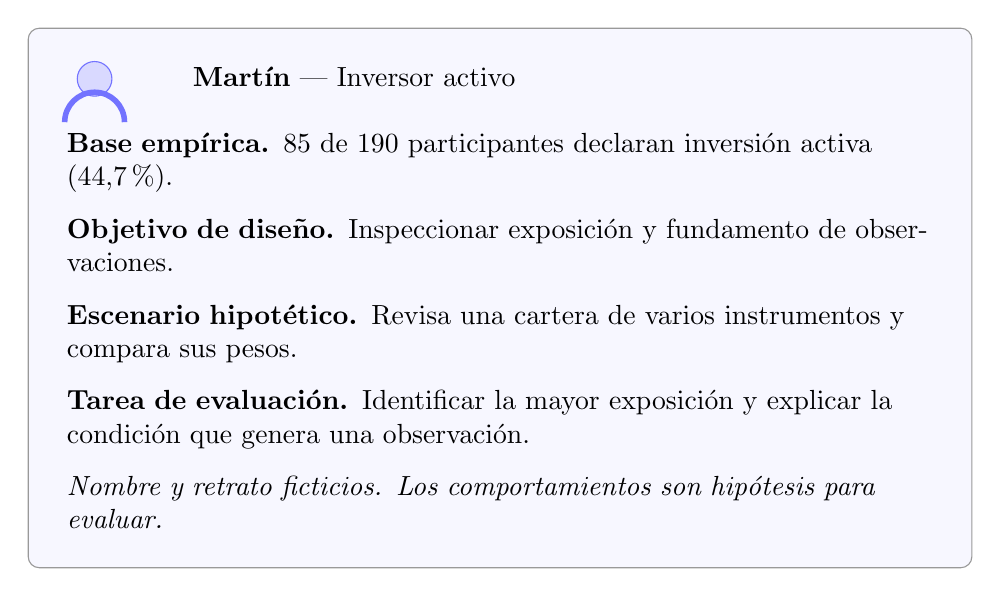
\begin{tikzpicture}
\node[draw=black!40,rounded corners,fill=blue!3,text width=11cm,inner sep=14pt,align=left] (card) {\hspace{1.6cm}\textbf{Martín} --- Inversor activo\\[12pt]
\textbf{Base empírica.} 85 de 190 participantes declaran inversión activa (44,7\,\%).\\[7pt]
\textbf{Objetivo de diseño.} Inspeccionar exposición y fundamento de observaciones.\\[7pt]
\textbf{Escenario hipotético.} Revisa una cartera de varios instrumentos y compara sus pesos.\\[7pt]
\textbf{Tarea de evaluación.} Identificar la mayor exposición y explicar la condición que genera una observación.\\[7pt]
\textit{Nombre y retrato ficticios. Los comportamientos son hipótesis para evaluar.}};
\begin{scope}[shift={([xshift=0.85cm,yshift=-0.65cm]card.north west)}]
\draw[fill=blue!15,draw=blue!55] (0,0) circle (0.22);
\draw[draw=blue!55,line width=2pt] (-0.38,-0.55) arc[start angle=180,end angle=0,radius=0.38];
\end{scope}
\end{tikzpicture}
\caption{Persona usuaria: inversor activo. Fuente: elaboración propia.}\label{fig:persona-activo}
\end{figure}

\begin{figure}[ht]\centering
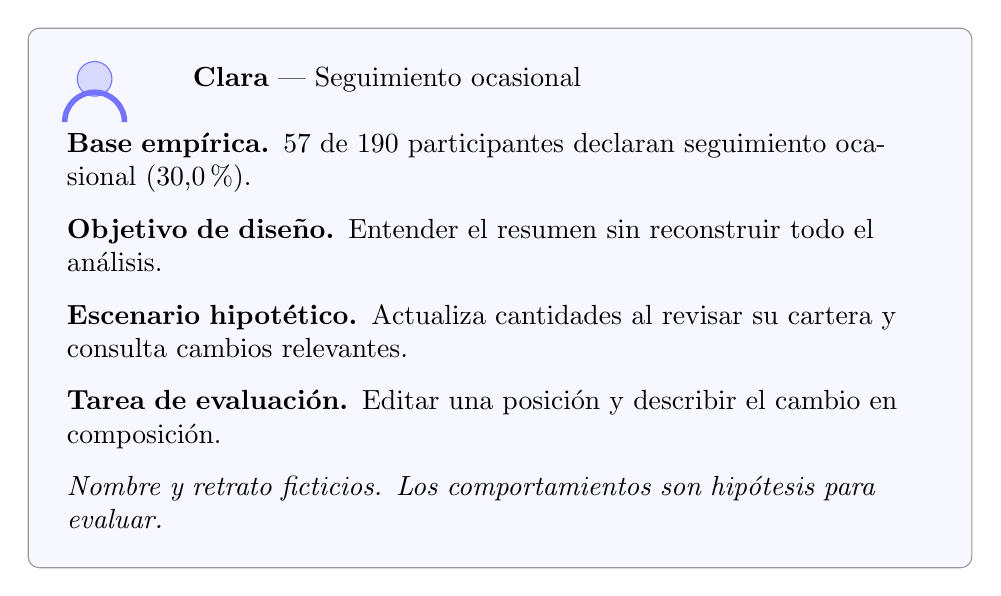
\begin{tikzpicture}
\node[draw=black!40,rounded corners,fill=blue!3,text width=11cm,inner sep=14pt,align=left] (card) {\hspace{1.6cm}\textbf{Clara} --- Seguimiento ocasional\\[12pt]
\textbf{Base empírica.} 57 de 190 participantes declaran seguimiento ocasional (30,0\,\%).\\[7pt]
\textbf{Objetivo de diseño.} Entender el resumen sin reconstruir todo el análisis.\\[7pt]
\textbf{Escenario hipotético.} Actualiza cantidades al revisar su cartera y consulta cambios relevantes.\\[7pt]
\textbf{Tarea de evaluación.} Editar una posición y describir el cambio en composición.\\[7pt]
\textit{Nombre y retrato ficticios. Los comportamientos son hipótesis para evaluar.}};
\begin{scope}[shift={([xshift=0.85cm,yshift=-0.65cm]card.north west)}]
\draw[fill=blue!15,draw=blue!55] (0,0) circle (0.22);
\draw[draw=blue!55,line width=2pt] (-0.38,-0.55) arc[start angle=180,end angle=0,radius=0.38];
\end{scope}
\end{tikzpicture}
\caption{Persona usuaria: seguimiento ocasional. Fuente: elaboración propia.}\label{fig:persona-ocasional}
\end{figure}

\begin{figure}[ht]\centering
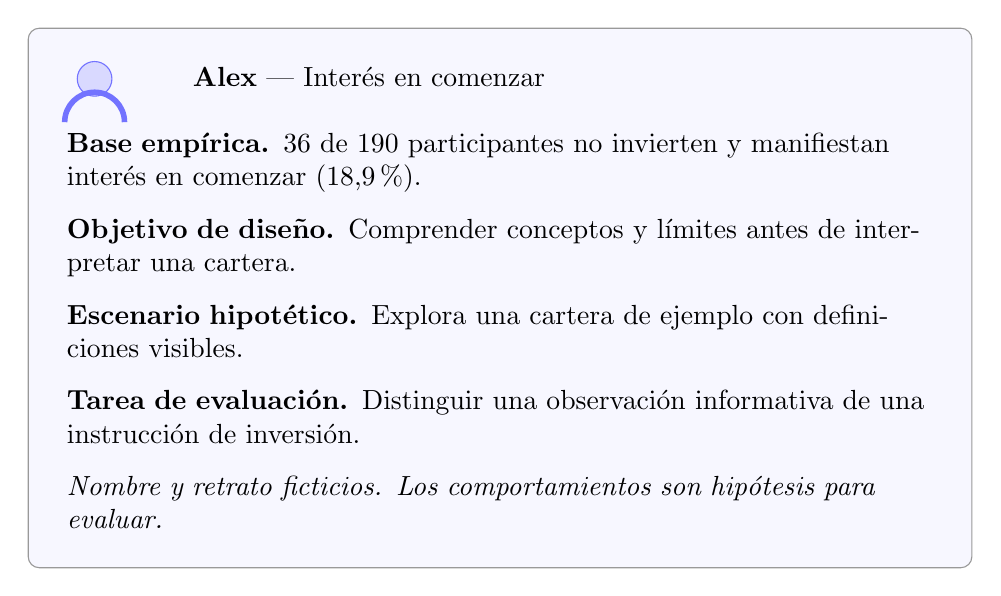
\begin{tikzpicture}
\node[draw=black!40,rounded corners,fill=blue!3,text width=11cm,inner sep=14pt,align=left] (card) {\hspace{1.6cm}\textbf{Alex} --- Interés en comenzar\\[12pt]
\textbf{Base empírica.} 36 de 190 participantes no invierten y manifiestan interés en comenzar (18,9\,\%).\\[7pt]
\textbf{Objetivo de diseño.} Comprender conceptos y límites antes de interpretar una cartera.\\[7pt]
\textbf{Escenario hipotético.} Explora una cartera de ejemplo con definiciones visibles.\\[7pt]
\textbf{Tarea de evaluación.} Distinguir una observación informativa de una instrucción de inversión.\\[7pt]
\textit{Nombre y retrato ficticios. Los comportamientos son hipótesis para evaluar.}};
\begin{scope}[shift={([xshift=0.85cm,yshift=-0.65cm]card.north west)}]
\draw[fill=blue!15,draw=blue!55] (0,0) circle (0.22);
\draw[draw=blue!55,line width=2pt] (-0.38,-0.55) arc[start angle=180,end angle=0,radius=0.38];
\end{scope}
\end{tikzpicture}
\caption{Persona usuaria: interés en comenzar. Fuente: elaboración propia.}\label{fig:persona-principiante}
\end{figure}

\FloatBarrier

\anexo{Casos de prueba y evidencia técnica}\label{annex:casos-prueba}

Las matrices de este anexo provienen de la reverificación del 13 de octubre de 2026, descrita en la Subsubsección~\ref{sec:reverificacion-octubre13}. La Tabla~\ref{tab:casos-ejecutados} reúne los casos CP, que ejecutan los servicios reales con repositorios, caché y respuestas externas simulados. Cada identificador coincide con el registro JSON y el programa indicados en la Subsección~\ref{sec:entorno-pruebas}. \enquote{Satisfactorio} significa únicamente que pasan todas las comprobaciones de ese caso; la aceptación del requisito completo es una conclusión aparte. En la ejecución del 8 de octubre, la primera pasada detecta tres defectos y la repetición posterior a las correcciones satisface los 21 casos; la reverificación los satisface en una sola pasada.

\begingroup
\small
\setlength{\tabcolsep}{4pt}
\begin{longtable}{>{\raggedright\arraybackslash}p{0.11\textwidth}>{\raggedright\arraybackslash}p{0.20\textwidth}>{\raggedright\arraybackslash}p{0.29\textwidth}>{\raggedright\arraybackslash}p{0.29\textwidth}}
\caption{Casos técnicos ejecutados y resultados. Fuente: elaboración propia a partir del registro automatizado.}\label{tab:casos-ejecutados}\\
\hline
\textbf{Caso / Req.} & \textbf{Entrada} & \textbf{Resultado esperado} & \textbf{Resultado obtenido} \\
\hline
\endfirsthead
\hline
\textbf{Caso / Req.} & \textbf{Entrada} & \textbf{Resultado esperado} & \textbf{Resultado obtenido} \\
\hline
\endhead
\hline
\endfoot
CP01\newline RF4/\allowbreak RNF2 & Sin posiciones. & Valor, HHI y número efectivo 0; sin dominante. & \textbf{Satisfactorio}. Coincide. \\ \hline
CP02\newline RF4/\allowbreak RNF2 & 2 unidades a precio 10. & Valor 20; peso 1; HHI 10000; número efectivo 1. & \textbf{Satisfactorio}. Coincide. \\ \hline
CP03\newline RF3/\allowbreak RF4/\allowbreak RNF2 & Cantidades 2/3/4; precios 10/20/5. & Pesos 0,2/0,6/0,2; HHI 4400; número efectivo 2,3; Global 0,8. & \textbf{Satisfactorio}. Coincide dentro de tolerancia en pesos; sumas de grupos iguales a 1. \\ \hline
CP04\newline RF4 & Cuatro pesos 0,25. & HHI 2500, moderado; número efectivo 4. & \textbf{Satisfactorio}. Coincide. \\ \hline
CP05\newline RF4 & Diez pesos 0,1. & HHI 1000, bajo. & \textbf{Satisfactorio}. Coincide. \\ \hline
CP06\newline RF2 & Alta 2; suma 3; edición a 7; baja. & Cantidades 5 y 7; lista final vacía. & \textbf{Satisfactorio}. Coincide. \\ \hline
CP07\newline RF2 & Ticker desconocido; cantidades 0, -1 y NaN. & Excepciones con estado 400. & \textbf{Satisfactorio}. Rechaza todas las entradas ensayadas. \\ \hline
CP08\newline RNF4 & Dos propietarios, mismo ticker. & Lecturas separadas; edición y baja ajenas rechazadas. & \textbf{Satisfactorio}. Excepciones 404; cantidad original conservada. \\ \hline
CP09\newline RF1/\allowbreak RNF5 & Correo con espacios y mayúsculas; contraseña; alta repetida. & Normalización; hash bcrypt factor 12; inicio de sesión válido; rechazos 401 y 409. & \textbf{Satisfactorio}. Coincide. \\ \hline
CP10\newline RNF4 & Token ausente, inválido y vencido. & Guard rechaza los tres con estado 401. & \textbf{Satisfactorio}. Coincide. \\ \hline
CP11\newline RF1 & Token firmado para usuario 2. & Guard acepta y asigna identificador 2. & \textbf{Satisfactorio}. Coincide. \\ \hline
CP12\newline RF6 & Análisis vacío. & Lista de observaciones vacía. & \textbf{Satisfactorio}. Coincide. \\ \hline
CP13\newline RF6 & Mayor posición de 25 y 26 por ciento. & No activar y activar conc-top, respectivamente. & \textbf{Satisfactorio}. Coincide. \\ \hline
CP14\newline RF6 & Cripto de 25, 40 y 41 por ciento. & Sin exp-cripto; atención; alerta. & \textbf{Satisfactorio}. Coincide. \\ \hline
CP15\newline RF8 & Mitad acciones y mitad cripto, sin evidencia reciente. & Escenarios y escenarios con fuentes vacíos; sin rendimientos supuestos. & \textbf{Satisfactorio}. Coincide; sustituye la comprobación de impactos fijos del 8 de octubre. \\ \hline
CP16\newline RF6 & Cartera con tecnología, cripto y energía. & Todas las observaciones generadas incluyen evidencia de tipo regla. & \textbf{Satisfactorio}. Se incorpora la regla; pasa la repetición. \\ \hline
CP17\newline RF5/\allowbreak RNF7 & Ambos proveedores fallan. & Conservar el conjunto local sin cambios. & \textbf{Satisfactorio}. Coincide. \\ \hline
CP18\newline RF5 & Fear \& Greed 22; dominancia 61,25. & Actualizar a 22 y 61,3; traducir Miedo extremo. & \textbf{Satisfactorio}. Coincide. \\ \hline
CP19\newline RF5/\allowbreak RNF7 & Alternative.me responde; CoinGecko falla. & Evitar origen global en vivo al conservar componentes locales. & \textbf{Satisfactorio}. Origen mixto y procedencia por componente. \\ \hline
CP20\newline RF5/\allowbreak RNF7 & Fear \& Greed 999; CoinGecko falla. & Descartar 999 y conservar respaldo 34. & \textbf{Satisfactorio}. Descarta 999 y conserva 34. \\ \hline
CP21\newline RNF7 & Dos lecturas consecutivas; fallos externos. & Solo dos llamadas externas en total; TTL solicitado 900 s. & \textbf{Satisfactorio}. Coincide; no prueba expiración real. \\ \hline
\end{longtable}
\endgroup

Todas las entradas son sintéticas y las huellas del código quedan guardadas en el registro JSON. Los casos CP usan dobles de prueba; las Tablas~\ref{tab:casos-integracion} a~\ref{tab:casos-playwright} cubren HTTP con persistencia real, el recorrido web automatizado, seguridad y pruebas unitarias adicionales. Todas las filas provienen de ejecuciones automatizadas.

\Needspace{8\baselineskip}
\section*{Integración HTTP y persistencia real}
La Tabla~\ref{tab:casos-integracion} lista los casos IT, ejecutados por HTTP contra PostgreSQL y Redis reales.
\begin{longtable}{>{\raggedright\arraybackslash}p{0.12\textwidth}>{\raggedright\arraybackslash}p{0.67\textwidth}p{0.12\textwidth}}
\caption{Casos de integración HTTP con persistencia real. Fuente: elaboración propia a partir del registro automatizado.}\label{tab:casos-integracion}\\
\hline
\textbf{Caso} & \textbf{Comprobación} & \textbf{Estado}\\\hline\endfirsthead
\hline
\textbf{Caso} & \textbf{Comprobación} & \textbf{Estado}\\\hline\endhead
IT01 & Registro HTTP de dos cuentas persistidas y contraseña hasheada & Pasa \\\hline
IT02 & Inicio de sesión válido y rechazo de credenciales incorrectas & Pasa \\\hline
IT03 & Rutas privadas rechazan token ausente, inválido y vencido & Pasa \\\hline
IT04 & DTO HTTP rechaza cantidad cero, ticker desconocido y registro inválido & Pasa \\\hline
IT05 & CRUD HTTP persiste la cantidad cifrada en PostgreSQL & Pasa \\\hline
IT06 & Otra cuenta no lee, edita ni elimina posiciones ajenas & Pasa \\\hline
IT07 & Análisis HTTP coincide con precios persistidos & Pasa \\\hline
IT08 & Observaciones HTTP incluyen regla y procedencia individual & Pasa \\\hline
IT09 & Redis real conserva respuesta de señales y TTL & Pasa \\\hline
IT10 & FK rechaza posiciones sin propietario o con usuario inexistente & Pasa \\\hline
IT11 & Eliminación HTTP de posición persistida & Pasa \\\hline
IT12 & Baja exige contraseña y elimina cuenta y posiciones & Pasa \\\hline
IT13 & Token previo de cuenta borrada queda inutilizable & Pasa \\\hline
IT14 & 30 consultas de análisis y observaciones con 100 posiciones reales & Pasa \\\hline
IT15 & Limpieza de segunda cuenta sin afectar cuenta demo & Pasa \\\hline
\end{longtable}

\section*{Recorrido web automatizado}
La Tabla~\ref{tab:casos-web} reúne los casos UI y X del recorrido de navegador sobre la interfaz vigente.
\begin{longtable}{>{\raggedright\arraybackslash}p{0.12\textwidth}>{\raggedright\arraybackslash}p{0.67\textwidth}p{0.12\textwidth}}
\caption{Casos del recorrido web automatizado sobre la interfaz vigente. Fuente: elaboración propia a partir del registro automatizado.}\label{tab:casos-web}\\
\hline
\textbf{Caso} & \textbf{Comprobación} & \textbf{Estado}\\\hline\endfirsthead
\hline
\textbf{Caso} & \textbf{Comprobación} & \textbf{Estado}\\\hline\endhead
UI01 & Ruta privada redirige al acceso conservando el destino & Pasa \\\hline
UI02 & Registro con consentimiento abre cartera vacía y emite la cookie de sesión HttpOnly y SameSite estricta & Pasa \\\hline
UI03 & Carga de AAPL, BTC y XLE, edición de AAPL y persistencia tras recargar & Pasa \\\hline
UI04 & Resumen y Riesgo: observación de energía con regla, datos y fuente visibles & Pasa \\\hline
UI04b & Escenarios sin rendimientos supuestos cuando falta evidencia & Pasa \\\hline
UI05 & Sin desborde horizontal en nueve pantallas con 390, 768 y 1440 px & Pasa \\\hline
UI06 & Eliminar posición con confirmación & Pasa \\\hline
UI07 & Cerrar sesión, revocar el token anterior, error de inicio de sesión y nuevo acceso & Pasa \\\hline
UI08 & Baja de cuenta: formulario validado, sesión cerrada y acceso posterior rechazado & Pasa \\\hline
UI09 & Sin errores de página ni de consola inesperados durante el recorrido & Pasa \\\hline
X01 & Otra cuenta no ve ni modifica posiciones ajenas & Pasa \\\hline
X02 & Mutaciones con origen ausente o ajeno rechazadas & Pasa \\\hline
X03 & El proxy exige sesión y solo expone rutas permitidas & Pasa \\\hline
X04 & Ticker inexistente, cantidad cero, negativa o con letras rechazados & Pasa \\\hline
X05 & Señales con fuente, fecha y origen visibles & Pasa \\\hline
X06 & El inicio de sesión tolera espacios y mayúsculas en el correo & Pasa \\\hline
X07 & Exportación de las posiciones propias & Pasa \\\hline
X08 & Detalle de activo y ruta inexistente sin errores & Pasa \\\hline
X09 & Treinta cargas de pantallas en tres anchos sin errores de consola & Pasa \\\hline
X10 & La baja de una cuenta no afecta a otra & Pasa \\\hline
X11 & Contraseña incorrecta en la baja muestra el error y conserva la sesión; falla en la primera pasada y pasa tras la corrección & Pasa \\\hline
\end{longtable}

\Needspace{12\baselineskip}
\section*{Comprobaciones web adicionales}
La Tabla~\ref{tab:casos-web-extra} detalla las comprobaciones sobre aspectos que el recorrido principal no abarca.
\begin{longtable}{>{\raggedright\arraybackslash}p{0.12\textwidth}>{\raggedright\arraybackslash}p{0.67\textwidth}p{0.12\textwidth}}
\caption{Comprobaciones web adicionales. Fuente: elaboración propia a partir del registro automatizado.}\label{tab:casos-web-extra}\\
\hline
\textbf{Caso} & \textbf{Comprobación} & \textbf{Estado}\\\hline\endfirsthead
\hline
\textbf{Caso} & \textbf{Comprobación} & \textbf{Estado}\\\hline\endhead
E01 & Página de privacidad accesible sin sesión, con su contenido y sin errores de consola & Pasa \\\hline
E02 & Modo mantenimiento: las páginas y la API responden 503 y la privacidad sigue disponible & Pasa \\\hline
E03 & Sesión vencida: aviso en el acceso y retorno al acceso con una cookie inválida & Pasa \\\hline
E04 & Tras 20 intentos de acceso, la web informa el límite de solicitudes sin romperse & Pasa \\\hline
E05 & Mostrar y ocultar la contraseña funciona y se anuncia al lector de pantalla & Pasa \\\hline
E06 & Accesibilidad con axe-core (WCAG 2.1 A y AA): sin violaciones graves ni críticas en 12 pantallas y dos anchos; falla en la primera pasada y pasa tras la corrección & Pasa \\\hline
E07 & Cabeceras de seguridad: CSP con nonce, sin caché, tipo de contenido y marcos & Pasa \\\hline
E08 & Sin conexión, la web informa el error, conserva el dato y se recupera al volver & Pasa \\\hline
E09 & Cartera: ordenar por cantidad cambia el orden de las filas & Pasa \\\hline
E10 & Acceso solo con teclado: el orden de tabulación llega al botón y Enter inicia sesión & Pasa \\\hline
E12 & Cerrar sesión en una pestaña invalida la otra & Pasa \\\hline
E14 & Redirección tras el acceso: respeta rutas internas y rechaza destinos externos & Pasa \\\hline
E15 & Un nombre con HTML se muestra como texto y no ejecuta código & Pasa \\\hline
E16 & La cuenta de pruebas se elimina al finalizar & Pasa \\\hline
\end{longtable}

\section*{Seguridad, IA y programación regional}
Los casos de la Tabla~\ref{tab:casos-seguridad} se ejecutan en local, con HTTP, PostgreSQL y Redis aislados; las fuentes externas y el modelo se simulan.
\begin{longtable}{>{\raggedright\arraybackslash}p{0.12\textwidth}>{\raggedright\arraybackslash}p{0.67\textwidth}p{0.12\textwidth}}
\caption{Casos de seguridad, IA y programación regional. Fuente: elaboración propia a partir del registro automatizado.}\label{tab:casos-seguridad}\\
\hline
\textbf{Caso} & \textbf{Comprobación} & \textbf{Estado}\\\hline\endfirsthead
\hline
\textbf{Caso} & \textbf{Comprobación} & \textbf{Estado}\\\hline\endhead
SEC01 & Contraseña mínima, consentimiento y alta de cuentas & Pasa \\\hline
SEC02 & Cookie web HttpOnly y SameSite sin token en el cuerpo & Pasa \\\hline
SEC03 & Rechazo de mutaciones con origen ausente o ajeno & Pasa \\\hline
SEC04 & Cifrado autenticado y aleatorio de cantidades & Pasa \\\hline
SEC05 & Aislamiento de lectura, edición y baja por propietario & Pasa \\\hline
SEC06 & Ocho acumulaciones concurrentes sin pérdida & Pasa \\\hline
SEC07 & Rechazo de campos extra, exceso y precisión inválida & Pasa \\\hline
SEC08 & Revocación de token y cookie al cerrar sesión & Pasa \\\hline
SEC09 & Cabeceras, no-cache e identificador de solicitud & Pasa \\\hline
AI01 & Rechazo de citas e identificadores no suministrados & Pasa \\\hline
AI02 & Filtro de antigüedad, futuro, URL y HTML externo & Pasa \\\hline
AI03 & Abstención sin cotización y sin llamada al modelo & Pasa \\\hline
SCH01 & DST, cierre anticipado, feriado sin sesión y cripto & Pasa \\\hline
SCH02 & Idempotencia, alerta por tenencia y datos mínimos a IA & Pasa \\\hline
SCH03 & Lectura aislada y retiro de consentimiento de alertas & Pasa \\\hline
SCH04 & Solicitud manual con sesión, solo con tenencias propias y deduplicada por hora & Pasa \\\hline
SCH08 & Estado por activo visible solo para quien lo solicita: cola, éxito y fallo & Pasa \\\hline
SCH07 & Último informe visible; el push manual omite el silencio solo para el solicitante & Pasa \\\hline
SEC12 & Estado global sin símbolos de solicitudes privadas & Pasa \\\hline
SCH05 & Fallo de una fuente sin bloquear otros activos; reintento sin duplicar & Pasa \\\hline
PUSH01 & Reinicio ambiguo sin reenvío; fallo de recibos sin interrumpir la limpieza & Pasa \\\hline
SEC10 & Exportación legible y baja de posiciones, alertas y dispositivos & Pasa \\\hline
SEC11 & Rate limit de autenticación con Retry-After & Pasa \\\hline
\end{longtable}

\Needspace{12\baselineskip}
\section*{Pruebas unitarias y de integración adicionales}
Los doce conjuntos de la Tabla~\ref{tab:casos-unitarios} pertenecen a la API y se ejecutan con el ejecutor de pruebas de Node.js. Cada fila indica cuántas pruebas tiene el conjunto; todas pasan.
\begin{longtable}{>{\raggedright\arraybackslash}p{0.30\textwidth}>{\raggedright\arraybackslash}p{0.50\textwidth}r}
\caption{Pruebas unitarias y de integración adicionales. Fuente: elaboración propia a partir del registro automatizado.}\label{tab:casos-unitarios}\\
\hline
\textbf{Conjunto} & \textbf{Cobertura} & \textbf{Pruebas}\\\hline\endfirsthead
\hline
\textbf{Conjunto} & \textbf{Cobertura} & \textbf{Pruebas}\\\hline\endhead
Correo de cuenta & Privacidad, reintentos, uso único, vencimiento y revocación de sesión & 1 \\\hline
Logos de activos & Dominios y formatos permitidos & 1 \\\hline
Cotizaciones de mercado & Caducidad, concurrencia acotada y fechas antiguas informadas & 3 \\\hline
Oportunidades & Con fuente y sin probabilidad inventada; informes inválidos rechazados & 4 \\\hline
Oportunidades (integración) & PostgreSQL aislado: seguimiento, alertas y eliminación en cascada & 1 \\\hline
Actualización de cotizaciones & Consulta manual al proveedor & 1 \\\hline
Publicación & Identidad firmada del limitador y cortes cripto sin calendario bursátil & 2 \\\hline
Investigación y descubrimiento & Indicadores diarios, series inválidas, importación segura y macroeconomía & 9 \\\hline
Evidencia de escenarios & Escenarios con fuente exacta, sin impacto inventado en la cartera & 2 \\\hline
Señales en vivo & Caída total o parcial sin semilla y sin shocks supuestos en producción & 5 \\\hline
Señales en español & Traducción que conserva las fuentes y rechaza identificadores desconocidos & 3 \\\hline
Instantánea de valuación & Aislamiento, vigencia, modificación de cantidades y eliminación ante fallo & 1 \\\hline
\end{longtable}

\Needspace{12\baselineskip}
\section*{Suite Playwright}
Sin ajustes, la suite solo pasa 4 de 26 pruebas. La Tabla~\ref{tab:casos-playwright} muestra el resultado después de actualizar los textos y selectores que habían quedado desactualizados y de agregar la prueba de baja con contraseña incorrecta.
\begin{longtable}{>{\raggedright\arraybackslash}p{0.34\textwidth}>{\raggedright\arraybackslash}p{0.12\textwidth}>{\raggedright\arraybackslash}p{0.14\textwidth}}
\caption{Suite Playwright. Fuente: elaboración propia a partir del registro automatizado.}\label{tab:casos-playwright}\\
\hline
\textbf{Conjunto} & \textbf{Pruebas} & \textbf{Satisf.}\\\hline\endfirsthead
\hline
\textbf{Conjunto} & \textbf{Pruebas} & \textbf{Satisf.}\\\hline\endhead
Flujos de la aplicación & 17 & 17 \\\hline
Consola del navegador & 4 & 4 \\\hline
Publicación & 1 & 1 \\\hline
Claridad visual & 1 & 1 \\\hline
Oportunidades & 1 & 1 \\\hline
Cuenta compartida & 1 & 1 \\\hline
Correo de la cuenta & 1 & 1 \\\hline
Baja con contraseña incorrecta & 1 & 1 \\\hline
\end{longtable}

\anexo{Protocolo de evaluación con usuarios}\label{annex:protocolo-usuarios}

Este protocolo se aplicó entre el 21 y el 23 de octubre de 2026; los resultados se presentan al final del anexo y se analizan en la Subsección~\ref{sec:pruebas-usabilidad}. Propone una evaluación exploratoria con cinco personas del público objetivo, ajenas al equipo y al tutor. De cada participante se registran experiencia previa, dispositivo, versión evaluada y un código anónimo (U01--U05). Al comenzar se explica la finalidad académica y se pide consentimiento para tomar notas; grabar la sesión exige un consentimiento aparte. La persona puede abandonar en cualquier momento sin consecuencias.

\textbf{Preparación.} El moderador comprueba que el servidor responde y usa cuentas de prueba, sin nombres, correos ni carteras personales. Lee cada tarea en voz alta sin indicar dónde hacer clic. Si ayuda, anota en qué consistió la ayuda y marca la tarea como asistida. Un silencio o un clic no se anotan como comprensión. Al terminar, elimina la cuenta de prueba si la persona no completó esa tarea.

\textbf{Tareas para leer al participante.} Las cantidades y los activos son solo ejemplos para la prueba y no constituyen una propuesta de inversión.
\begin{enumerate}
\item Crear una cuenta ficticia e ingresar. Cargar 2 AAPL, 0,1 BTC y 100 XLE. Corregir AAPL a 3 y comprobar que el cambio se conserva al volver a entrar.
\item Consultar el análisis e indicar cuál es la mayor posición y qué peso representa. Explicar qué interpreta del indicador de concentración.
\item Abrir la explicación relacionada con energía. Indicar qué condición la activa, qué datos utiliza y de dónde proviene el contexto. Mostrar en pantalla la evidencia que respalda la respuesta.
\item Identificar una señal externa y una de demostración. Explicar la diferencia entre fecha del dato y fecha de consulta. Abrir los escenarios con fuentes y decir si lo que se muestra es un pronóstico o una condición posible con su fuente.
\item Eliminar BTC, cerrar y abrir la sesión y, finalmente, eliminar la cuenta y sus posiciones mediante la confirmación prevista.
\end{enumerate}

\textbf{Registro por tarea.} Por cada participante se completa una ficha con: código; fecha; dispositivo; inicio y fin; resultado (éxito sin ayuda, éxito con ayuda o tarea no completada); errores observados; ayuda brindada; respuesta literal; comentario posterior. Una ficha vacía es solo el formulario y no cuenta como sesión.

\textbf{Criterios de análisis.} La tarea 3 se considera comprendida si la persona identifica sin ayuda la condición de exposición energética superior al 5\,\% junto con un evento relacionado, y reconoce la fuente local de demostración. El umbral exploratorio es cuatro de cinco participantes. Para las demás tareas se informan por separado éxito, tiempo, errores y ayuda. Todos los participantes se mantienen en el denominador, cualquiera sea su resultado; los abandonos y los registros incompletos se explican. Con cinco personas, los resultados describen la experiencia de uso: no admiten generalización estadística ni dicen nada sobre rendimiento financiero.

\textbf{Cierre.} Al final se pregunta qué parte resultó confusa, qué información faltó y qué decisiones cree la persona que la herramienta puede apoyar y cuáles no. Las respuestas se anotan con sus palabras antes de sintetizarlas. Cada hallazgo se traduce en un cambio concreto y en una nueva comprobación.

\section*{Resultados}
La Tabla~\ref{tab:sesiones-participantes} identifica las sesiones y la Tabla~\ref{tab:sesiones-matriz} el resultado de cada tarea por participante, con las abreviaturas S (sin ayuda), A (con ayuda) y N (no completada). Como en el servicio publicado no se activó la regla de exposición energética, la tarea 3 se evaluó sobre la observación de posición dominante y el criterio de comprensión pasó a ser identificar sin ayuda la condición del 25\,\% y su origen en la propia cartera. Los escenarios con fuentes no estaban disponibles y esa parte de la tarea 4 no se evaluó. El registro completo, con horas, errores, ayuda y respuestas literales, está en \texttt{evidence/2026-10-sesiones-usuarios/sesiones\_usuarios.csv}.

\begin{table}[ht]
\centering\small\renewcommand{\arraystretch}{1.15}
\caption{Sesiones realizadas. Fuente: registro de las sesiones.}\label{tab:sesiones-participantes}
\begin{tabular}{llllll}\hline
\textbf{Código} & \textbf{Fecha} & \textbf{Modalidad} & \textbf{Dispositivo} & \textbf{Segmento} & \textbf{Duración}\\\hline
U01 & 21/10/2026 & presencial & web (notebook) & activo & 23 min\\
U02 & 21/10/2026 & videollamada & app Android & activo & 25 min\\
U03 & 22/10/2026 & presencial & web (notebook) & activo & 25 min\\
U04 & 22/10/2026 & presencial & app iOS & ocasional & 41 min\\
U05 & 23/10/2026 & videollamada & web (teléfono) & principiante & 50 min\\\hline
\end{tabular}
\end{table}

\begin{table}[ht]
\centering\small\renewcommand{\arraystretch}{1.15}
\caption{Resultado por tarea y participante. Fuente: registro de las sesiones.}\label{tab:sesiones-matriz}
\begin{tabular}{lccccc}\hline
\textbf{Tarea} & \textbf{U01} & \textbf{U02} & \textbf{U03} & \textbf{U04} & \textbf{U05}\\\hline
1. Cuenta, carga y edición & S & S & A & A & A\\
2. Mayor posición y concentración & S & S & S & A & A\\
3. Explicar una observación & S & A & S & A & N\\
4. Fuentes y fechas & A & S & A & N & N\\
5. Eliminar posición y baja de cuenta & S & A & S & A & N\\\hline
\end{tabular}
\end{table}

Respuestas literales en la tarea 3, que decide el criterio de comprensión:
\begin{itemize}
\item U01 (sin ayuda): \enquote{Este es por peso de una posición. Dice que si supera el 25\,\%, lo marca. No habla de una noticia sobre Bitcoin.}
\item U02 (con ayuda): \enquote{Es porque tengo más del veinticinco por ciento en una sola cosa. No porque el precio haya caído ahora.}
\item U03 (sin ayuda): \enquote{La regla salta arriba de 25\,\% en un activo, y el porcentaje se calcula con la cartera que armé. Esto no es una orden de vender.}
\item U04 (con ayuda): \enquote{Entonces no es que bajó Bitcoin. Es que tengo mucho de la misma cosa, más de 25\,\%. Está calculado con mi cartera.}
\item U05 (no completada): \enquote{Dice veinticinco por ciento, pero no sé si es lo que tengo que vender o el máximo que puedo comprar.}
\end{itemize}

Respuestas de cierre: U01, \enquote{lo más confuso fueron las fechas; la parte de concentración se entiende mejor cuando abrís la explicación}; U02, \enquote{lo que me desconcertó fue que la advertencia parecía de mercado y era de mi cartera}; U03, \enquote{me gustó ver el motivo del aviso; la parte de escenarios necesita dejar más claro cuándo no hay un informe}; U04, \enquote{cargar se puede; los términos de Riesgo me cuestan, y las fechas también}; U05, \enquote{para ver cuánto tengo está bueno; para entender esas alertas necesitaría que me lo expliquen más fácil}.

